%% Copernicus Publications Manuscript Preparation Template for LaTeX Submissions
%% ---------------------------------
%% This template should be used for copernicus.cls
%% The class file and some style files are bundled in the Copernicus Latex Package, which can be downloaded from the different journal webpages.
%% For further assistance please contact Copernicus Publications at: production@copernicus.org
%% https://publications.copernicus.org/for_authors/manuscript_preparation.html


%% Please use the following documentclass and journal abbreviations for preprints and final revised papers.

%% 2-column papers and preprints
\documentclass[journal abbreviation, manuscript]{copernicus}



%% Journal abbreviations (please use the same for preprints and final revised papers)


% Advances in Geosciences (adgeo)
% Advances in Radio Science (ars)
% Advances in Science and Research (asr)
% Advances in Statistical Climatology, Meteorology and Oceanography (ascmo)
% Annales Geophysicae (angeo)
% Archives Animal Breeding (aab)
% ASTRA Proceedings (ap)
% Atmospheric Chemistry and Physics (acp)
% Atmospheric Measurement Techniques (amt)
% Biogeosciences (bg)
% Climate of the Past (cp)
% DEUQUA Special Publications (deuquasp)
% Drinking Water Engineering and Science (dwes)
% Earth Surface Dynamics (esurf)
% Earth System Dynamics (esd)
% Earth System Science Data (essd)
% E&G Quaternary Science Journal (egqsj)
% European Journal of Mineralogy (ejm)
% Fossil Record (fr)
% Geochronology (gchron)
% Geographica Helvetica (gh)
% Geoscience Communication (gc)
% Geoscientific Instrumentation, Methods and Data Systems (gi)
% Geoscientific Model Development (gmd)
% History of Geo- and Space Sciences (hgss)
% Hydrology and Earth System Sciences (hess)
% Journal of Bone and Joint Infection (jbji)
% Journal of Micropalaeontology (jm)
% Journal of Sensors and Sensor Systems (jsss)
% Magnetic Resonance (mr)
% Mechanical Sciences (ms)
% Natural Hazards and Earth System Sciences (nhess)
% Nonlinear Processes in Geophysics (npg)
% Ocean Science (os)
% Polarforschung - Journal of the German Society for Polar Research (polf)
% Primate Biology (pb)
% Proceedings of the International Association of Hydrological Sciences (piahs)
% Scientific Drilling (sd)
% SOIL (soil)
% Solid Earth (se)
% The Cryosphere (tc)
% Weather and Climate Dynamics (wcd)
% Web Ecology (we)
% Wind Energy Science (wes)


%% \usepackage commands included in the copernicus.cls:
%\usepackage[german, english]{babel}
%\usepackage{tabularx}
%\usepackage{cancel}
%\usepackage{multirow}
%\usepackage{supertabular}
%\usepackage{algorithmic}
%\usepackage{algorithm}
%\usepackage{amsthm}
%\usepackage{float}
%\usepackage{subfig}
%\usepackage{rotating}


\usepackage{comment} 
\usepackage{enumerate}

\begin{document}

\title{The XSO framework (v0.1) and Phydra library (v0.1) for a flexible, reproducible and integrated plankton ecosystem modeling environment in Python} 


% \Author[affil]{given_name}{surname}
\Author[1,2]{Benjamin}{Post}
\Author[3]{Esteban}{Acevedo-Trejos}
\Author[4]{Andrew D.}{Barton}
\Author[1,2]{Agostino}{Merico}



\affil[1]{Department of Theoretical Ecology \& Modelling, Leibniz Centre for Tropical Marine Research (ZMT), Bremen, Germany}
\affil[2]{Department of Physics and Earth Science, Jacobs University Bremen, Germany}
\affil[3]{GFZ German Research Centre for Geosciences, Potsdam, Germany}
\affil[4]{Scripps Institution of Oceanography and Section of Ecology, Behavior and Evolution, University of California San Diego, La Jolla, CA, United States}

%% The [] brackets identify the author with the corresponding affiliation. 1, 2, 3, etc. should be inserted.

%% If an author is deceased, please mark the respective author name(s) with a dagger, e.g. "\Author[2,$\dag$]{Anton}{Aman}", and add a further "\affil[$\dag$]{deceased, 1 July 2019}".

%% If authors contributed equally, please mark the respective author names with an asterisk, e.g. "\Author[2,*]{Anton}{Aman}" and "\Author[3,*]{Bradley}{Bman}" and add a further affiliation: "\affil[*]{These authors contributed equally to this work.}".


\correspondence{Benjamin Post (benjamin.post@leibniz-zmt.de)}


\runningtitle{phydra v1}

\runningauthor{Post}





\received{}
\pubdiscuss{} %% only important for two-stage journals
\revised{}
\accepted{}
\published{}

%% These dates will be inserted by Copernicus Publications during the typesetting process.

\firstpage{1}

\maketitle

\begin{abstract}

Plankton ecosystem modeling is a critical tool for understanding the processes that shape marine ecosystems and their impacts on global biogeochemical cycles. These models can be of variable ecological, physiological and physical complexity. The source codes of a good deal of published plankton community models are not publicly available, and in many cases their mathematical structures and technical implementations are not flexible enough to be easily modified, thus hampering transparency, reproducibility of results, and the ease of adoption by novel users. Here we present Phydra, an open-source library for plankton ecosystem modelling, and Xarray-simlab-ODE (XSO), a modular framework for efficient, flexible, and reproducible model development based on ordinary differential equations, both written in Python. Phydra provides pre-built models and model components that can be modified and assembled to develop marine ecosystem models of various levels of ecological complexity. The components can be created, adapted and modified using standard variables types provided by the XSO framework. XSO is embedded in the Python scientific ecosystem and is natively compatible with many tools for prototyping and analyzing models and for visualizing model results. 
To demonstrate the range of applicability and how Phydra and XSO can be used to develop and execute models, we present three model applications: (1) a highly simplified chemostat setting, (2) a NPZD ecosystem model in an open-ocean physical setting, and (3) a complex size-structured ecosystem model that resolves 50 phytoplankton and 50 zooplankton with parameters determined by allometric relationships. The applications presented here are available open-source in interactive Jupyter notebooks and can be used by the scientific community to build, modify, run, and test plankton community models based on differential equations for a diverse range of scientific pursuits.

\end{abstract}


\copyrightstatement{Phydra and XSO are based on other open-source efforts and published with MIT-3 licences for open access and fair usage.} %% This section is optional and can be used for copyright transfers.

%%% added Section for editing purposes, later simply use \introduction
\section{Introduction}
%\introduction  %% \introduction[modified heading if necessary]


% Introductory paragraph, spelling out the issue, end with: therefore we present Phydra/XSO!
Scientists have used mathematical models to advance our understanding of marine ecosystems for more than 80 years \citep{Sverdrup1953OnPhytoplankton, Fasham1990a, Follows2007EmergentOcean, Acevedo-Trejos2016, Gentleman2002a}. Early models comprising a few ordinary differential equations describing phytoplankton populations in a simplified physical setting \citep{Evans1985ACycles, Fasham1990a} have matured into detailed descriptions of multiple trophic levels that are run in complex three-dimensional general circulation models (GCMs) \citep[e.g.][]{Dutkiewicz2020DimensionsDiversity}. While plankton community models in some cases lack biological realism \citep{Smith2014}, and often suffer from poorly constrained model parameters and comparisons to observations \citep{Anderson2005}, they have been enormously important in developing our understanding of the mechanisms that shape plankton biogeography \citep[e.g.][]{Follows2007EmergentOcean}, phenology \citep[e.g.][]{Taylor1993SeasonalNitrogen}, and biodiversity \citep[e.g.][]{Barton2010b, Acevedo-Trejos2015c}, as well as links between ecosystems and biogeochemical cycles \citep[e.g.][]{Fasham1990a, Sarmiento1998SimulatedWarming, Dutkiewicz2009}.

%% Benny: I am unsure with the following paragraph (or sentence snippets), as I am not sure what exactly I am trying to say. I feel like mentioning Fortran, and how unintuitive those models are, but perhaps that is unfair. This paragraph seems crucial as it should be as specific as possible about the problem we are trying to solve. Do you have any idea how to best structure it? Some of this could be better placed in the discussion perhaps, but then what stays in the Introduction?
Despite this progress, we argue that plankton ecosystem models are often inflexible, overly complicated or inaccessible, which can obfuscate valuable research and present a high barrier of entry for non-specialists or students. Existing model code is rarely reused beyond the development teams \citep{Belete2017AnTesting}. Whilst many large models use legacy code that is difficult to integrate, resulting in "good knowledge bound in outdated code" \citep{Argent2004AnSemantics}. This particularly creates challenges when attempting to integrate models across domains, e.g. linking ecological models to sophisticated physical models \citep{Koralewski2019CouplingModels}, or when validating or calibrating models \citep{Steenbeek2021MakingPerspective}. 

Following the integrated environmental modeling approach, we should create tools for marine ecosystem modeling that are interoperable (i.e. communicate directly) with tools for data analysis and model evaluation \citep{Laniak2013IntegratedFuture}. 

Model formulations should be treated as hypotheses to be tested \citep{Franks2009}, so ideally our modeling tools allow for rapid prototyping and refactoring. 

To date most global circulation models and large marine ecosystem models are written in the highly efficient, but less commonly used programming language Fortran. Domain-specific researchers proficient in Fortran 

For example, the ERSEM marine ecosystem model implementation provides some flexibility to modify and experiment with model structures via markup language files or Python interfaces, but the general formulations are hard-coded in Fortran scripts \citep{Butenschon2016}. The limnological FABM-PCLake model was rewritten to allow for a more modular structure \citep[][]{Schnedler-Meyer2022WaterModel}. 

Modern, interpreted programming languages commonly used for data analysis applications (e.g. Python) have evolved the capabilities to efficiently support advanced numerical computations \citep{Lin2012}. This is showcased by Veros, a global circulation model (GCM) written in Python \citep{Hafner2018VerosPython}. The Python ecosystem and Jupyter Notebooks in particular \citep{Kluyver2016JupyterWorkflows}, have shown to be a useful tool for collaborative modeling workflows \citep[e.g. eWaterCycle platform,][]{Hut2022TheCollaboration}. 


There is a diversity of approaches to aquatic ecosystem models, and frameworks used
\citep{Janssen2015ExploringPerspective} <- actually provides systematic list of frameworks used (!)


- make model formulation more accessible for non-specialists! XSO/Phydra no replacement, but an added tool simplifying model construction
%%%%%



% <State in one clean sentence to goal of the new model framework.> 
To efficiently test and answer ecological and biogeochemical questions using marine ecosystem models, we need modeling tools that: (1) are easy to use, (2) are completely open-source, (3) allow flexible and granular control of model structure, and (4) are conducive to scientific collaboration via an open and extensible framework. These are the motivations that lead us to develop the novel XSO framework and Phydra library in the programming language Python. 

% <Provide 2-3 sentences of HIGH level summary of what XSO and Phydra do.> 
The XSO framework offers a set of building blocks for developing computational models based on ordinary differential equations. XSO is used as the basis of the marine ecosystem models contained in the Phydra library. The foundational framework facilitates the modification of model structure, components, dimensionality and parameterization. The ultimate goal is to provide usability and flexibility in line with popular Python data analysis and visualization tools, such as Pandas, Xarray and Matplotlib. The XSO framework depends on functionality from these packages and provides direct interoperability for an integrated modeling environment.

In the next section, we present the usage of the XSO framework and structure of the Phydra library, including the steps of an exemplary model development workflow. We show the utility of the tool-set in three exemplary model applications: (1) a basic NP chemostat model, (2) an NPZD model in a slab physical setting, adapted from \citet{Anderson2015c}, and (3) a complex size-resolved model in a simple box setting, adapted from \citet{Banas2011b}. These models form the basis of the first release of the Phydra library. We then discuss the architecture of the framework, current limitations and possible future developments.



% I commented out the glossary, because it doesn't really make sense in it's current state!
\begin{comment}
\subsection{Glossary}
We use the following terms with their respective definitions in this paper. We acknowledge that these terms can be ambiguous or cryptic in an inter-disciplinary context, and want to clarify our intended meaning within this text and the context of the presented code.

% IN order to make this section actually useful, I should only explain terms in the scope of this manuscript, and give examples.. e.g. Decorators: @xso.component and @xso.flux()
\begin{itemize}
    \item  \textit{Framework}: A framework is a set of predefined building blocks. More specifically in our case, the XSO framework provides Python classes and functions, that serve as the foundation for building ODE-based models. By utilizing the framework a user does not have to start from scratch, but can rely on existing functionality and compatibility, to build their specific application.
    
    \item  \textit{Library}: A library is a collection of pre-written code, that can directly be used within an application. The Phydra library provides a set of fully formed model components and entire models that utilize the XSO framework.

    \item  \textit{Decorator}:
    In Python, a decorator is a special type of function that allows you to modify or extend the behavior of another function or class. Decorators are applied to other functions or classes using the @ symbol, and they wrap the behavior of the original function or class with additional functionality. The two important decorator functions within the XSO framework is the class decorator \texttt{@xso.component} and the function decorator \texttt{@xso.flux}.
 
    \item  \textit{Attribute}:
    In Python, an attribute is a variable defined within a class. It is accessible through the object initialized from the class. The \textit{variable types} provided by XSO that are defined as attributes are: \textit{variables}, \textit{parameters} and \textit{forcings}.

    \item  \textit{Method}:
    In Python, a method is a function that is associated with an object and can be used to perform operations on the object's data. Methods are defined within a class and are called on instances of the class. Within the XSO framework, the \textit{flux} variable type is implemented as a method decorator. Additionally \textit{forcings} can use a method as a setup function.
    
    \item  \textit{Argument}:
    In Python, an argument is a value passed to a function or method when it is called. Arguments are used to provide input data to a function, method or decorator so that it can perform the desired operation. 
    
\end{itemize}

%% END OF INTRODUCTION

\end{comment}

 %% \ SECTION 2
\section{Descriptions of the XSO framework and the Phydra Library} \label{Section:phydrapackage}
%%% TWO-COLUMN FIGURES
%
%%f
\begin{figure*}[t]
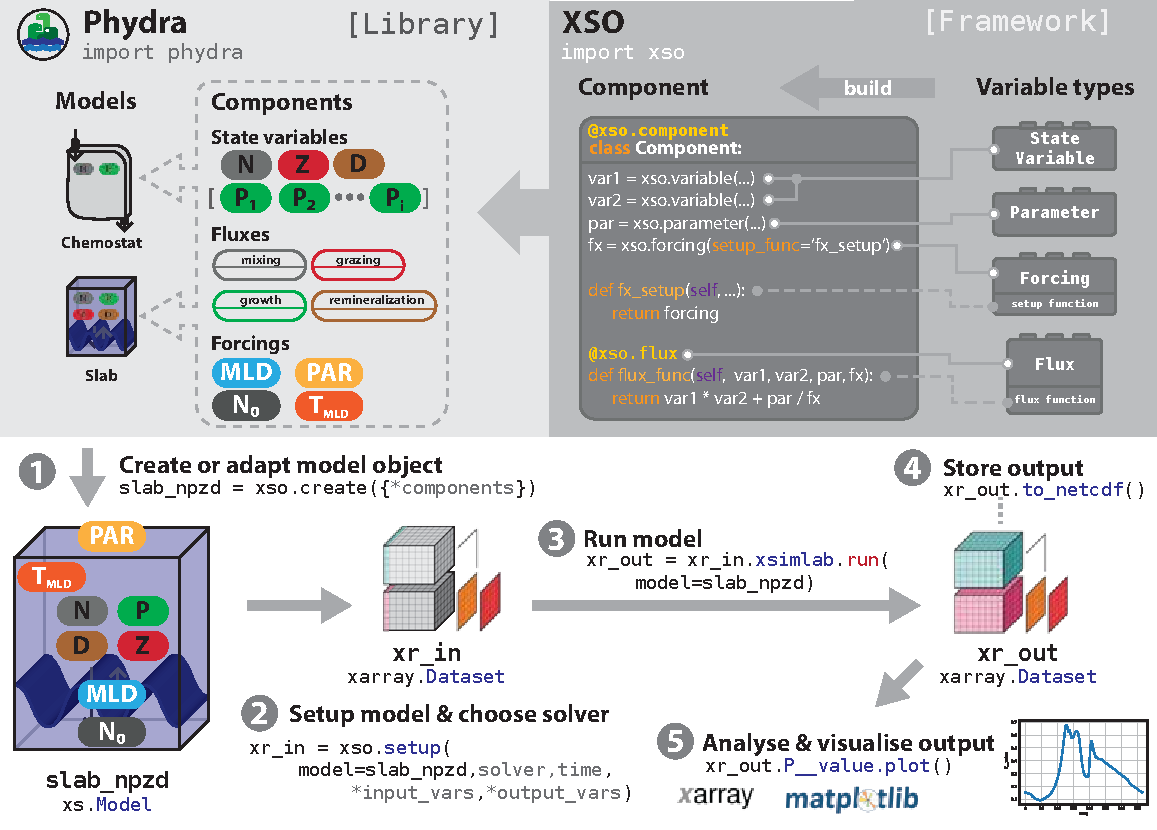
\includegraphics[width=12cm]{Figures/firstdraft_schematics/00_schematics_Package.pdf}
\caption{Schematic of package structure. XSO provides the framework. Phydra is a library of functional \textit{components} and pre-built \textit{model objects}, that can be used, extended, and modified. A typical workflow would consist of five steps. (1) Choose a pre-existing model, potentially remove or add \textit{components} or create a new model using \texttt{xso.create()}. (2) Create a \textit{model setup} by supplying the appropriate labels and parameters and solver to \texttt{xso.setup()}. The \textit{model setup} is an Xarray dataset. (3) To run the model, call the \textit{xsimlab.run()} method on the \textit{model setup}. Output is returned as a fully documented Xarray dataset. (4) These datasets can be easily stored or shared. (5) Xarray datasets are fully compatible to be analysed and visualised with the wealth of tools provided by the Python scientific ecosystem.}
\label{Figure:PhydraXSOPackageSchematics}
\end{figure*}

% 2nd Section: 
% Background, theoretical framework. Specifics here!
%The structure and functionality of Phydra and XSO and a simplified model development workflow are presented in Figure \ref{Figure:PhydraXSOPackageSchematics} and explained in more detail below. Interested researchers and potential users can find the most up-to-date documentation and code on GitHub (XSO: \url{https://github.com/ben1post/xarray-simlab-ode}, Phydra: \url{https://github.com/ben1post/phydra}). The documentation includes short guides on setting up a functional Python environment, including Jupyter Notebooks.

\subsection{The XSO framework} \label{Section:XSOFramework}


Xarray-simlab-ODE (XSO) is a Python framework that allows you to construct and customize models based on ordinary differential equations (ODEs) in a modular fashion. It is a non-opinionated framework, i.e. it does not provide a fixed notion of how the model should be implemented, instead it attempts to remove the redundant boiler-plate code, allowing a user to construct and work with ODE-based models in a flexible manner. XSO was developed as the technical foundation of the Phydra library, but is not limited to any particular domain and can be used to create ODE-based models of any type. The typical steps of a model development workflow are presented in figure \ref{Figure:PhydraXSOPackageSchematics}.

The XSO framework is an extension of Xarray-simlab \citep{Bovy2018Xarray-simlab:Interactively, Bovy2021Benbovy/xarray-simlab:0.5.0}, which itself provides a generic and highly flexible model development framework in Python. It relies on advanced Python functionalities, such as compact data classes and decorators (see the online-documentation for more details). Xarray-simlab provides a succinct set of functions and attributes to construct Python objects, that can interact as processes of a larger model. In addition to this interface, Xarray-simlab provides powerful data handling capabilities, storing model input and output as labelled multidimensional Xarray datasets \citep{Hoyer2017Xarray:Python}. Model output is thus directly compatible with a wealth of other Python tools for data analysis or visualisation and can be readily exported to the NetCDF file standard (amongst others).

Xarray-simlab has found fruitful applications, for example in landscape evolution modeling \citep{Bovy2021Fastscape-lem/fastscape:V0.1.0beta3} and plant growth modeling \citep{Vaillant2022TowardsDevelopment}. The Xarray-simlab framework is generic in that it provides only a step-wise execution of model processes and no concept of time. Our package, XSO, is technically a wrapper around Xarray-simlab, adding custom building blocks and backend code to allow a user to easily define and compute models based on differential equation.

Our objective in developing the XSO framework was to enable users to construct ODE-based models to be readily modified, particularly in regards to the dimensionality and number of state variables and processes involved. XSO provides an interface for iterative modifications, both to more complex and simpler model constructs. The building blocks provided by XSO are as follows:


% Should this list be perhaps a table, and more concise?
\begin{itemize}
    \item  \textbf{\textit{Variable types}}: These are the most granular elements of the framework, which directly correspond to the basic mathematical components of ODE-based models (e.g. state variables, parameters, forcing, and partial equations). XSO currently provides the following \textit{variable types}: 
    \begin{itemize}
        \item \texttt{xso.variable}: Defines a state variable in a \textit{component}, either locally or via reference in another \textit{component}.
        \item \texttt{xso.forcing}: Defines an external forcing as a constant or time-varying value, via an additional setup function. Can also be a reference to a forcing in another \textit{component}.
        \item \texttt{xso.parameter}: Defines a constant model parameter, either locally or via reference.
        \item \texttt{xso.flux}: Defines a mathematical term with the \textit{variable types} in the \textit{component}, and adds the term into the system of differential equations of the underlying model. The flux function decorator provides a group argument, that allows linking multiple fluxes flexibly between components.
    \end{itemize}
    These can be used to define variables in compact Python classes, to construct functional XSO \textit{components}. All of them can be defined with a variable number of dimensions (i.e. as a vector, array or matrix).

    \item \textbf{\textit{Components}}: These are the general building-blocks of a model that declare a subset of variables and define a specific set of mathematical functions computed for these variables during model runtime. More specifically, a \textit{component} refers to a Python class containing \textit{variable types} that is decorated with \texttt{@xso.component}. For example, a \textit{component} could define a specific nutrient uptake function, e.g. Monod-type phytoplankton growth on a single nutrient. The decorating function registers the \textit{variable types} within the framework, reducing boilerplate code and creating fully functional model building blocks. \textit{Components} can be reused within a model.
    
    \item \textbf{\textit{Model object}}: These are instances of the Model class provided by Xarray-simlab. They consist of an ordered, immutable collection of \textit{components}. A XSO \textit{model object} is created with a call to the function \texttt{xso.create()} by supplying a dictionary of model \textit{components} with their respective labels. \textit{Model objects} contain the \textit{components} relevant to a model and can be easily stored and shared. They do not contain custom parameterisation.

   \item \textbf{\textit{Model setup}}: This object is an Xarray dataset, that includes all relevant information needed at runtime, such as the \textit{model object}, solver algorithm to be used, as well as time steps and model parameterisation. A XSO \textit{model setup} is created with a call to the function \texttt{xso.setup()} and supplying the aforementioned information as arguments. At this step, the \textit{variable types} initialized in a \textit{component} must be supplied with a value, as well as a label that can be used to reference them in other \textit{components}. The model parameterisation is passed as a dictionary, with the \textit{component} labels used to create the \textit{model object} as keys.
\end{itemize}

The system of differential equations is constructed from the \textit{fluxes} using the labels supplied during model setup. The number of values in a defined dimension is flexible, but they have to match across the model in order for the model to run. 
When executing the model by calling the \texttt{xsimlab.run()} method of the \textit{model setup} and supplying the appropriate \textit{model object}, a "filled-out" Xarray dataset is returned containing model setup parameters, metadata and output.

%These design choices ensure that the effort required to construct a model is proportional to the desired level of complexity, models and \textit{components} can be easily modified to incorporate more complex formulations. We hope that this will encourage experimentation and inter-comparison of model performance across a range of complexities.

The XSO framework currently provides two solver algorithms: an adaptive step-size solver from the SciPy package (odeint) and a simple step-wise solver that is built into the backend Xarray-simlab framework. Apart from the technical limitations of the solver algorithm used, there are no restrictions on the dimensionality and number of \textit{variable types} used within a \textit{component} and no limitations to the levels of \textit{group} variables linking components to define a single ecosystem process. 


% DON'T REPEAT YOURSELF OVER AND OVER !
% Mention limitiation
% But highlight the flexibility and benefits
\begin{comment}
The XSO framework is currently limited to model applications based on ordinary differential equations (ODEs). With this limitation, conceptual marine ecosystem models still vary greatly in complexity. Our objective in developing the XSO framework was to enable users to construct ODE-based models to be readily modified, particularly in regards to the dimensionality and number of state variables and processes involved. XSO provides an interface for iterative modifications, both to more complex and simpler model constructs. The typical steps of a model development workflow are presented in figure \ref{Figure:PhydraXSOPackageSchematics}.


% SOLVER

% Computational Efficiency

% moot points:
- Xarray-simlab is so generic, that in fact it only provides a simple step wise execution of processes (no built-in concept of "time") and hard-coded links between processes. For marine ecosystem models, these are often based on differential equations and our goal of providing a modular flexible framework requires some way of flexible linkages between processes. XSO wraps Xarray-simlab, and adds that functionality.

- The backend code of XSO is separated from the user interface, and can be modified or completely rewritten without breaking functionality.
\end{comment}
    



\subsection{The Phydra library} \label{Section:PhydraLibrary}
Phydra is python package, that provides a library of marine ecosystem models built in a modular fashion using the XSO framework. The Phydra package provides a specific library for marine ecosystem modelling applications that establishes conventions and common usage.

 
The marine ecosystem models included in the Phydra package are available to the user at multiple hierarchical levels: as a library of pre-built XSO model \textit{components}, as pre-assembled \textit{model objects}, and as exemplary model simulations in interactive Jupyter notebooks. These levels are described below.

\begin{enumerate}
    \item \textbf{\textit{Components}}: The first version of the library will contain all \textit{components} used to create the three model applications presented in Section \ref{Section:UseCases}. The \textit{components} can be combined to zero-dimensional marine ecosystem models of variable complexity. The library follows common usage patterns and conventions. As long as the labelled model dimensions between \textit{components} match at model setup, all \textit{components} included in the Phydra library are compatible.
    
    \item \textbf{\textit{Model objects}}: The first release of phydra contains the \textit{model objects} defined in the three model applications presented in section \ref{Section:UseCases}. The \textit{model objects} can be imported from the library and can be readily setup, modified, and run by a user.
    
    \item \textbf{Example notebooks}: \textit{Model objects} only define the collection of \textit{components}. To run a model, the input parameters still need to be defined and supplied at runtime. The Phydra library comes with three fully documented model applications that are presented in interactive Jupyter notebooks. These notebooks show all steps from creating the \textit{model setup} object to analysing model output and provide a template for further exploration and experimentation with the provided marine ecosystem models.
    
\end{enumerate}

The open-source and extensible nature of Phydra and XSO enables users to customize and develop processes that accurately describe a particular ecosystem. In a collaborative effort to promote efficient, transparent, and reproducible marine ecosystem modeling, Phydra encourages users to contribute their own \textit{components} and \textit{models} to the core library. The Phydra library could potentially offer a comprehensive, well-documented, and peer-reviewed codebase for the scientific exploration of marine ecosystem models.







 %% \ SECTION 3
\section{Model applications} \label{Section:UseCases}

To showcase the utility of the XSO framework and Phydra library, we present three marine ecosystem model applications of varying complexity. For each application we present the mathematical model, the implementation within the XSO framework and some model results. To highlight the flexible nature of the model implementations in the XSO framework, we also show how one aspect of each model is modified.

For the first model application, we considered a simple model, whose implementation using the XSO framework is presented in full detail. For the presentation of the more complex models in use cases 2 and 3, we show only the \textit{component} structure and highlight additional technical aspects of the implementation. For all use cases the complete code, following the full development workflow from model creation to output visualization, is available publicly as interactive Jupyter notebooks in the Phydra repository (\url{https://github.com/ben1post/phydra/tree/master/examples}).

\subsection{Model application 1: phytoplankton growth in a chemostat}
%%f
\begin{figure}[t]
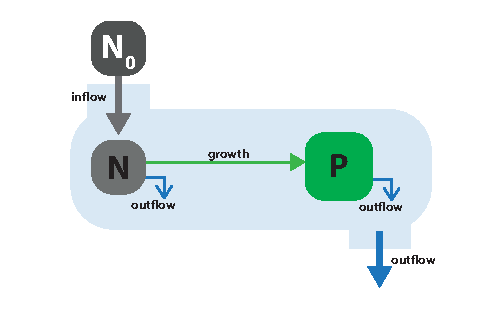
\includegraphics[width=8.3cm]{Figures/firstdraft_schematics/01_schematics_Chemostat.pdf}
\caption{Schematic of model application 1: phytoplankton $P$ feeding on a single nutrient $N$ in a flow-through system. The chemostat system includes an external nutrient input with concentration $N_0$. Both $N$ and $P$ flow out of the system at a constant dilution rate, $d$.}
\label{Figure:ModelSchematics_1}
\end{figure}

We first present a model of a phytoplankton population growing in a chemostat. Chemostats are a commonly used experimental setup for studying the dynamics of microorganisms under controlled laboratory settings. They are characterized by constant influx of medium containing nutrients and a constant outflow of the culture, with a rate of $d$ (units). With the appropriate medium and flow rates this allows a steady-state system to emerge, that is particularly useful for studying growth dynamics of microorganisms. Although the conditions of chemostat systems do not have a direct equivalent in nature, some oceanic upwelling systems can be approximated with such a simple model \citep{Haefner2005ModelingApplications}.

To showcase the flexibility and simplicity of the XSO framework, we considered two cases: (1) a constant nutrient input and (2) a sinusoidal nutrient input.

\subsubsection{Description}
The model is presented in Figure \ref{Figure:ModelSchematics_1}. It uses nitrogen as its currency (quantities are measured in units of \unit{µM \ N}, i.e. $\mu mol$ N $m^{-3}$), with state variables for dissolved nutrients ($N$) and phytoplankton ($P$). The physical environment is a flow-through system corresponding to a laboratory chemostat setup. Growth medium with nutrient concentration $N_0$ (\unit{µM \ N}) flows into the system at a rate $d$ (\unit{d^{-1}}). The model components ($N$ \& $P$) flow out of the system at that same rate.

Phytoplankton growth ($\mu$, \unit{d^{-1}}) is described by Monod kinetics \citep{Monod1942RecherchesBacteriennes}.
\begin{equation}
    \mu = \mu_{max} \frac{N}{k + N} 
\end{equation}
where $k$ (\unit{µM \ N}) is the half-saturation nutrient concentration, defined as the concentration at which half the maximum growth rate is achieved, $N$ is the ambient nutrient concentration, and $\mu_{max}$ (\unit{d^{-1}}) is the maximum growth rate achievable under perfect growth conditions.

The model equations are:

\begin{equation}
    \frac{d N}{d t} = 
    d (N_0 - N) % Nutrient input and output
    -  \mu_{max} \frac{N}{k_N + N} 
\end{equation}

%PHYTOPLANKTON
\begin{equation}
    \frac{d P}{d t} =
    \mu_{max} \frac{N}{k_N + N} 
    - d P
\end{equation}



\subsubsection{Implementation}

%%f
\begin{figure*}[t]
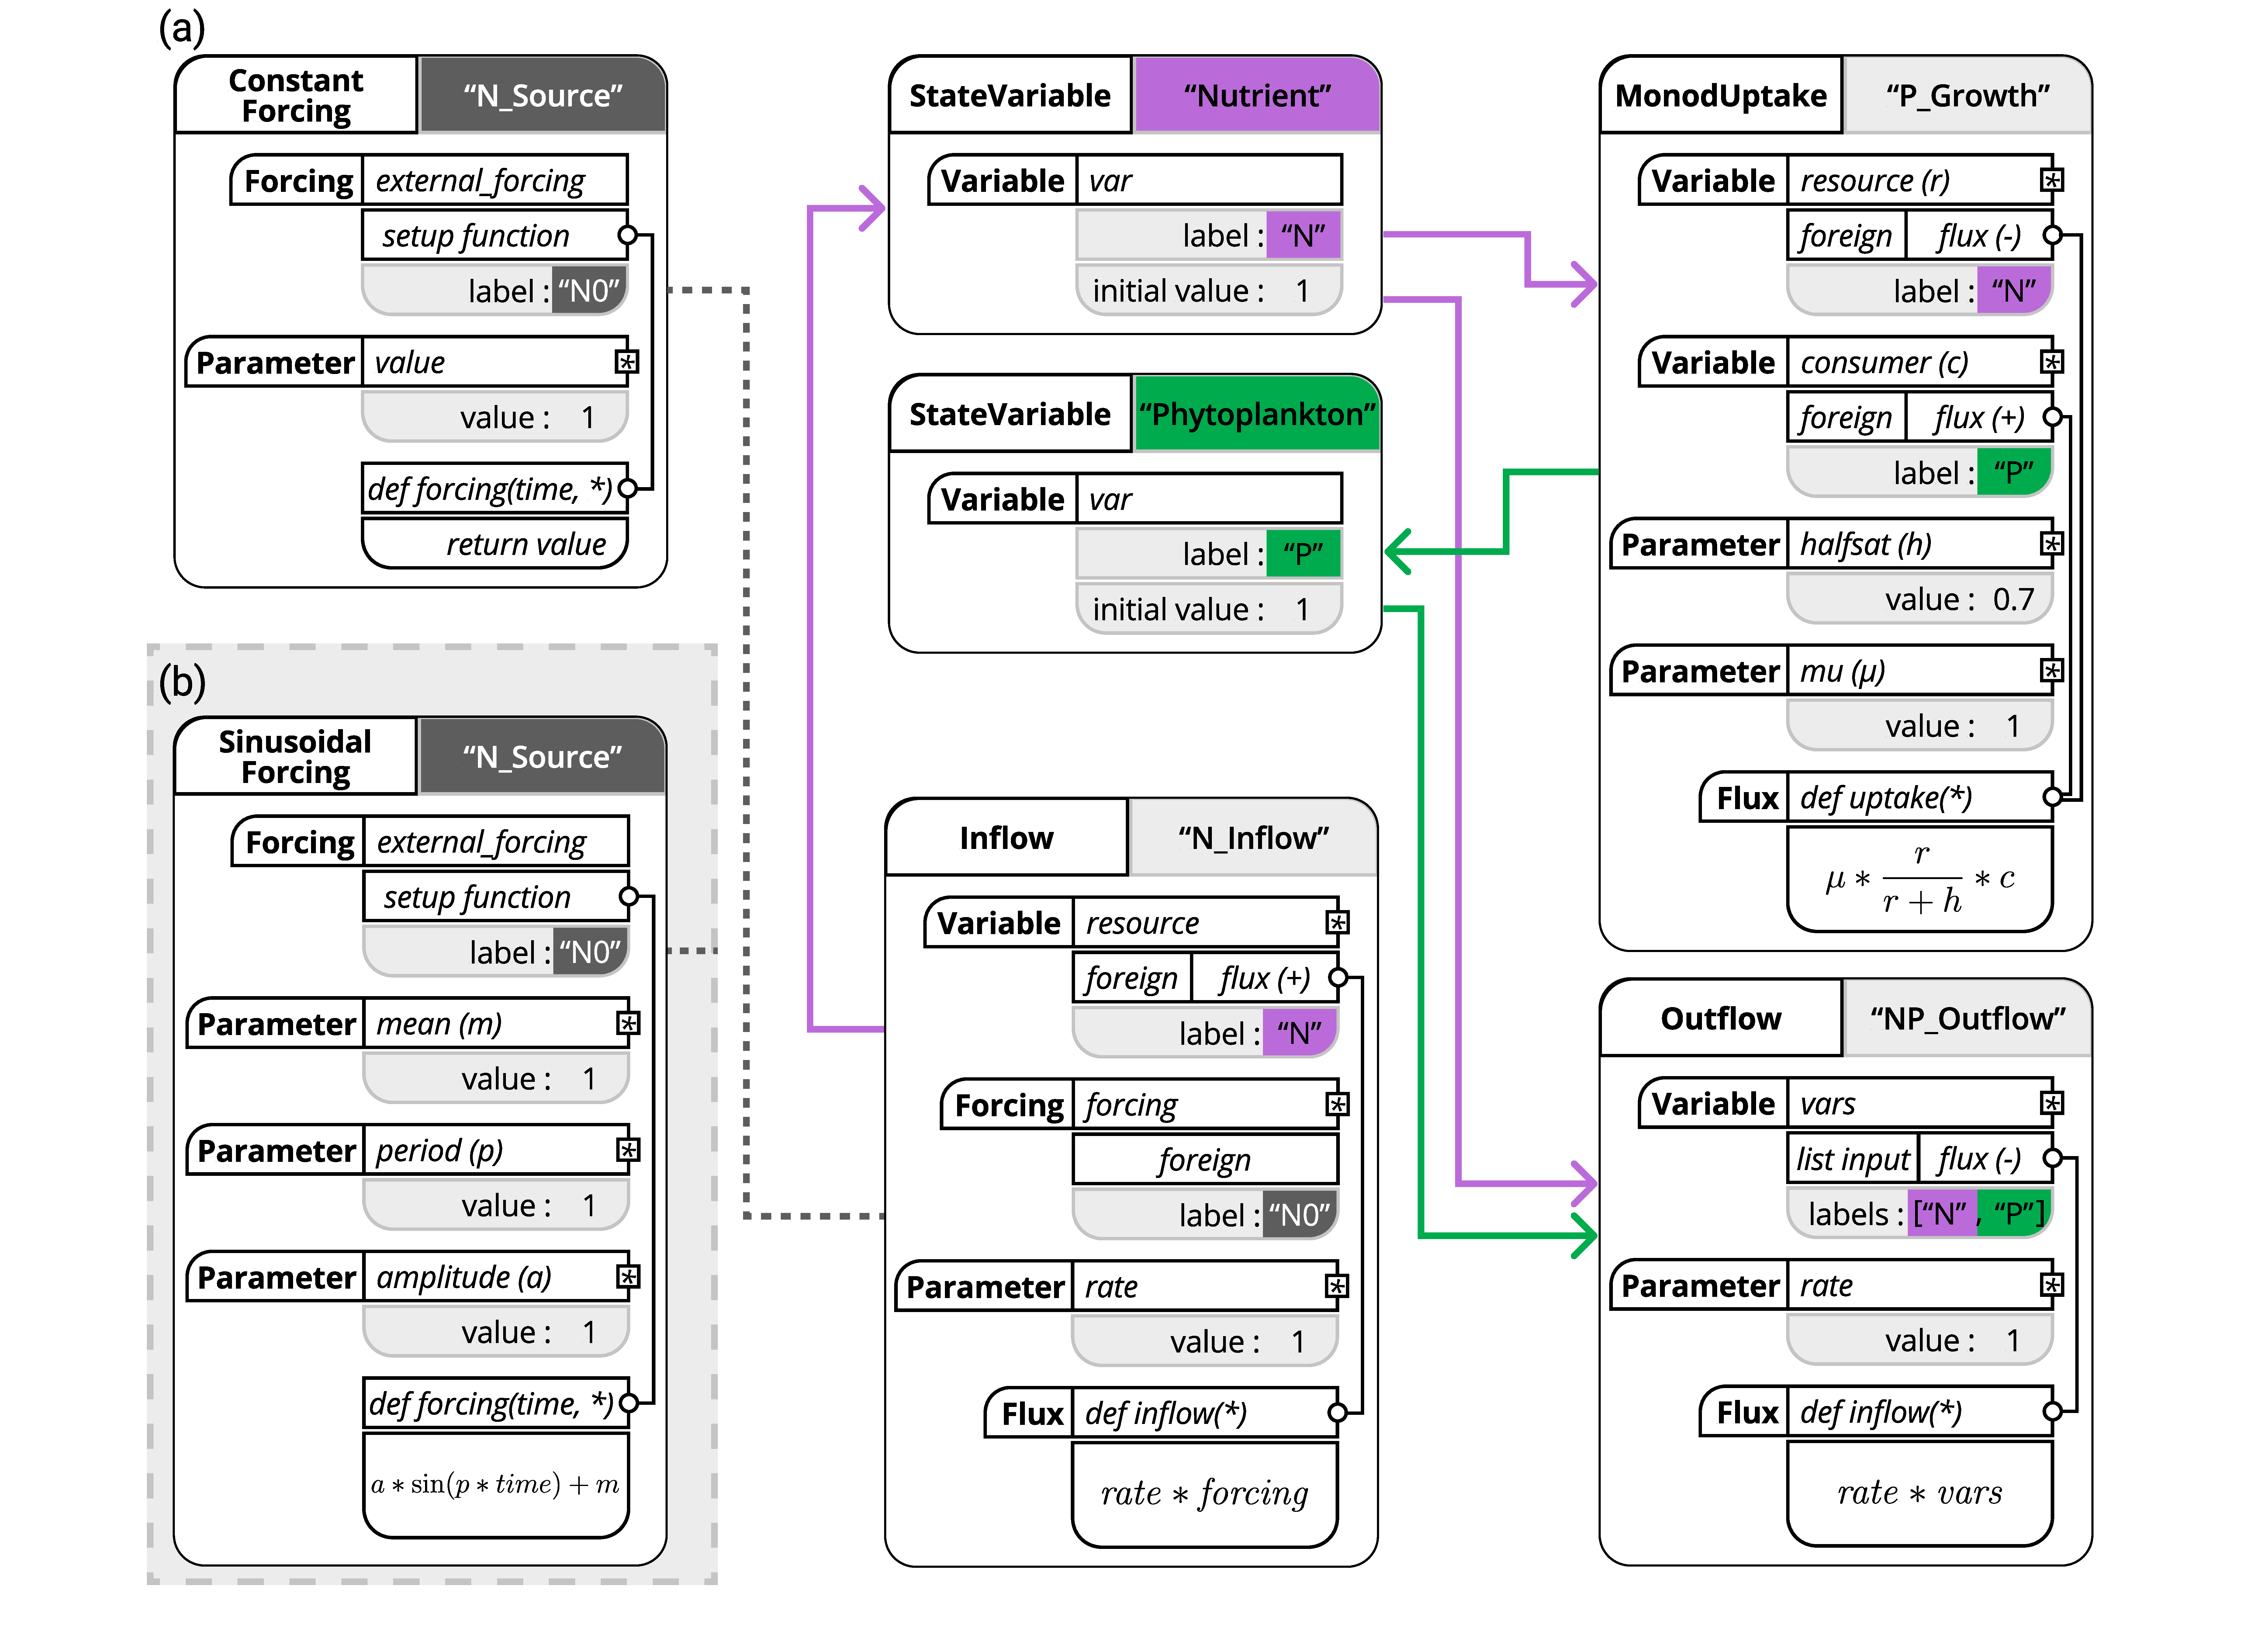
\includegraphics[width=15cm]{Figures/firstdraft_schematics/code_schematics/Chemostat.pdf}
\caption{A schematic representation of how model application 1 is implemented in the XSO framework and included in the Phydra library. Model setup with constant forcing (a) and with sinusoidal forcing (b). Structures in solid black are hard-coded into components. Labels of the different components are supplied at model creation. Gray boxes and the resulting links between components (shown as thick coloured arrows and dashed lines) are defined at model setup, via the supplied labels and parameters. The asterisk in the flux function input arguments references the variables, forcing and parameters defined within the same component, these local variables can be used in all functions (e.g. fluxes or forcing setup functions) within that same component.}
\label{Figure:CodeSchematics_1}
\end{figure*}

%%% TWO-COLUMN TABLE
%
%t
\begin{table*}[t]
\caption{Description of variables and parameters in the model application 1, the chemostat model. In addition to the values and units, we provide the variable names to compare in figure \ref{Figure:CodeSchematics_1}}
\begin{tabular}{l c c c r}
\tophline
Description & Symbol & Variable & Value & Units \\
\middlehline

Concentration of nitrogen in medium & $N$ & \texttt{N} & t(0) = 1 & \unit{µM \ N} \\
Concentration of phytoplankton in medium & $P$ & \texttt{P} & t(0) = 0.1 & \unit{µM \ N} \\
Nutrient concentration of external medium & $N_0$ & \texttt{N\_0} & 0.1 & \unit{µM \ N} \\
Maximum growth rate & $\mu_{max}$ & \texttt{mu\_max} & 1 & \unit{d^{-1}} \\
Dilution rate & $d$ & \texttt{rate} & 0.1 & \unit{d^{-1}}\\
Half-saturation constant &  $k_N$ & \texttt{halfsat} & 0.7 & \unit{µM \ N}\\

XXX Sinusoidal function (Mean, Period, Amplitude) &  $sin(x)$ & \texttt{xxx} & 2.7 & \unit{d^{-1}}\\

\bottomhline
\end{tabular}
\label{Table:UseCase1Parameters}
\end{table*}
%

In order to find a useful structuring of model components, we can separate the model into state variables, forcing, and fluxes. For state variables, we have nutrient ($N$) and phytoplankton ($P$). The only forcing is the nutrient concentration of the external medium ($N_0$), whether it is constant or variable. Three fluxes can be separately defined: (1) the inflow of the external medium, (2) $P$ growing on $N$, and (3) the outflow of both $N$ and $P$. The model was implemented using these 6 separate model components, as visualized in Figure \ref{Figure:CodeSchematics_1}.

To explore the basic dynamics, we chose standard parameters values (Table \ref{Table:UseCase1Parameters}). Initial values for $N$ and $P$ were set at 1 \unit{µM \ N} and 0.1 \unit{µM \ N}, respectively. The model was run for 100 days with a time step of 0.1 days.

In order to run the model with periodic forcing, we can simply exchange the forcing component from \texttt{ConstantForcing} to \texttt{SinusoidalForcing}. This specific component requires two more input parameters, but otherwise the model creation and setup remain the same. We can actually update the model object, by simply supplying the \texttt{SinusoidalForcing} component for the \texttt{"N\_inflow"} component via the \texttt{model.update\_processes()} method and updating the corresponding parameters via \texttt{model\_setup.update\_vars()} functions supplied by the Xarray-Simlab framework that XSO extends. Such functionality allows straightforward modification and testing of models.

\subsubsection{Results \& Discussion}

%%f
\begin{figure}[t]
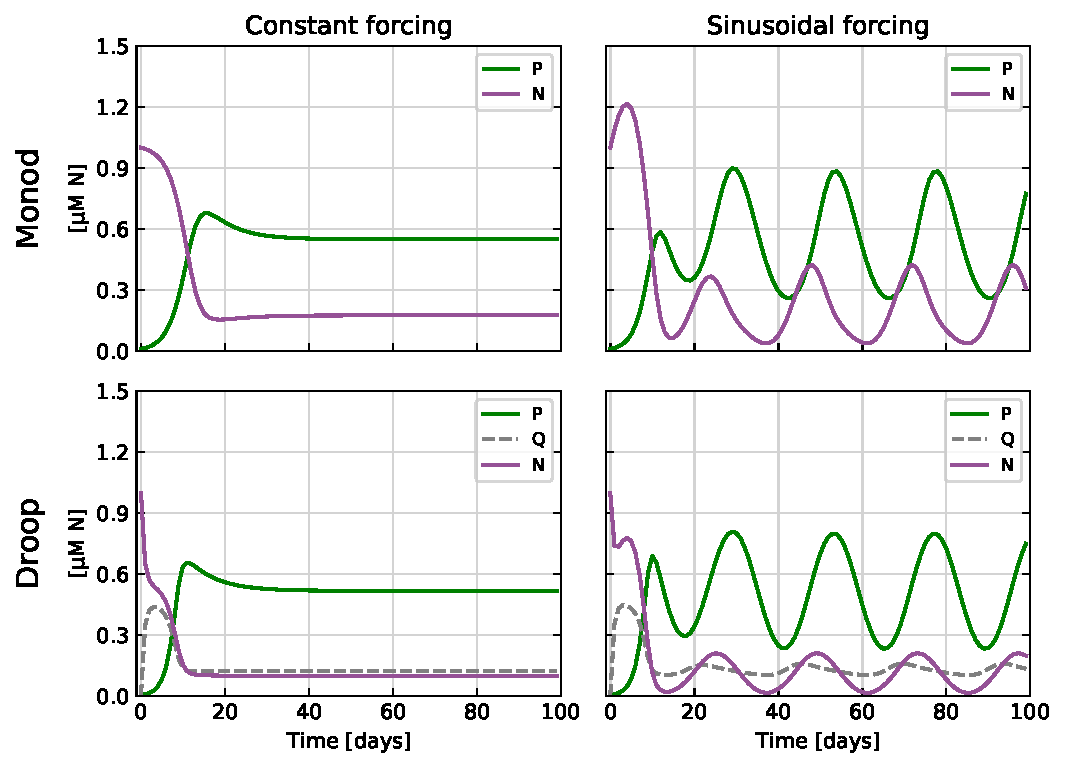
\includegraphics[width=8.3cm]{Figures/firstdraft_plots/01_chemostat_output.pdf}
\caption{Model output for the two chemostat model scenarios: (a) Constant forcing and (b) Sinusoidal forcing. In each case, the concentration of nutrient ($N$, purple) and phytoplankton ($P$, green) are shown through time.}
\label{Figure:ResultsChemostat}
\end{figure}

Figure \ref{Figure:ResultsChemostat} shows the two model runs performed, comparing constant nutrient concentration and periodically variable external nutrient concentration. Under constant forcing, the model quickly reaches a steady state, as nutrient supply and the resulting phytoplankton growth balances with the loss of nutrient and phytoplankton due to the constant outflux of medium. The periodically variable nutrient concentration creates oscillations in $P$ centred around 0.9 \unit{µM \ N}. In this highly simplified model, the results still show an interesting shift between the dynamics of nutrients and phytoplankton, as there is some time lag between the point in time, where all nutrients in the medium are consumed (due to a lack of replenishment from the variable nutrient source) and the peak in phytoplankton concentration.

This first model application represents a basic proof-of-concept that our presented library and framework can create expected results within a very simple model setup.




\subsection{Model application 2: NPZD slab model}
%%f
\begin{figure}[t]
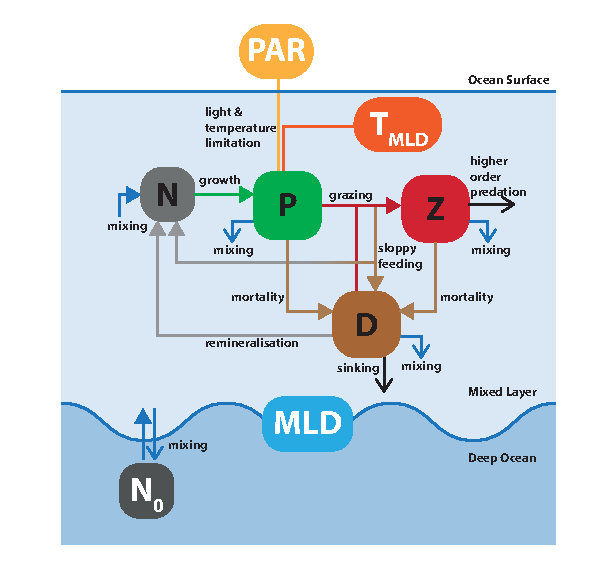
\includegraphics[width=8.3cm]{Figures/firstdraft_schematics/02_schematics_EMPOWER.pdf}
\caption{Model schematic of the NPZD slab model presented as a second application. The model structure is adapted
from \citet{Anderson2015c}. Boxes with black and white labels represent state variables and external forcing, respectively. Arrows indicate fluxes between state variables. The upper layer box contains the ecosystem model, with state variables for nutrients, phytoplankton, zooplankton and detritus. The curvy blue line represents the seasonally variable mixed layer depth (MLD) that defines the boundary between the upper layer and the inert deep ocean. The model presents a highly simplified, but efficient representation of an open ocean ecosystem.}
\label{Figure:ModelSchematics_2}
\end{figure}

The second model application describe a classic Nutrient-Phytoplankton-Zooplankton-Detritus (NPZD) ecosystem model embedded in a slab-ocean physical setting \citep[e.g.,][]{Evans1985ACycles, Fasham1990a}. "Slab" refers to a simplified zero-dimensional model of the oceanic upper mixed layer, that varies seasonally in depth above an inert deep layer. This classic model structure provides an efficient physical setting for more complicated ecosystem descriptions and is often used for teaching marine ecosystem modelling. The application is an implementation of the EMPOWER model, as was beautifully presented by \citet{Anderson2015c}. See Figure \ref{Figure:ModelSchematics_2} for a schematic of the model structure.

The NPZD slab model lends itself well to investigate the bulk nutrient dynamics in the upper ocean layer, as well as the export of biomass production. In the model, phytoplankton growth is affected by temperature, as well as light and nutrient availability. Phytoplankton are consumed by zooplankton predators, which are in turn subject to a higher order mortality (constituting grazing by higher trophic levels). Phytoplankton and zooplankton mortality, as well as grazing byproducts feed into a detrital pool, that is partially remineralised in the upper ocean. The movement and depth of the mixed layer has effects on all components. Nutrients are exchanged between the deep ocean and upper ocean across the mixed layer boundary. Phytoplankton, zooplankton and detritus experience a mixing loss term, with detritus additionally sinking at a constant rate out of the mixed layer.

Many NPZD-type models have been published over the years, with a plethora of formulations for the functional responses of the ecosystem components. The EMPOWER model was presented as an open-source model testbed, for example by providing various formulations for the treatment of light. \citet{Anderson2015c} provided a detailed discussion of light calculation and treatment, as this is a crucial and rather complex component of phytoplankton models. We follow their approach by considering two different light-attenuation algorithms that can be easily exchanged in our modular framework, to investigate the effects of more detailed treatment of light attenuation over water depth in comparison to a simplified integrated Lambert-Beer's law calculation. The EMPOWER model code was written as a monolithic R script, with some modifications allowed via user supplied flags, but no inherent modularity. We updated the model code to the modular and flexible XSO framework, allowing for greater adaptability and experimentation on this classic structure.

\subsubsection{Description}
% for EMPOWER move all description to supplementary, no need to explain everything again
% use simple plain english paragraph describing model
The model uses nitrogen as currency (quantities are measured in units of \unit{µM \ N}), with state variables for dissolved nutrients ($N$), phytoplankton ($P$), zooplankton ($Z$) and detritus ($D$). The water column is represented by two layers, where a biologically inert deep ocean box is situated below a homogeneously mixed upper box of variable depth that contains the ecosystem. The model structure, locations, and parameters are adapted from the EMPOWER model \citep{Anderson2015c}. For the definition of all symbols used here see Table \ref{appendix:table:usecase1symbols} and see \citet{Anderson2015c} for a more detailed discussion of model structure and formulation.

The model is driven by external forcing describing the depth of the upper mixed layer ($H$, \unit{m}), average temperature of the upper mixed layer ($T$, \unit{\degree C}), photosynthetically active radiation (PAR) at the surface ($I$; \unit{W m^{-2}}), and nutrient concentration in the deep layer ($N_0$, \unit{µM \ N}). 

% Nutrient dynamics
The deeper layer supplies nutrients to the upper layer, while other components are mixed to the deep layer and lost from the system. The magnitude of mixing is described by $K$ (\unit{d^{−1}}):

\begin{equation}
    K = \frac{h^{+} + \kappa}{H}
\end{equation}

Where $\kappa$ (\unit{m \ d^{−1}}) represents constant diffusive mixing. Variable mixing is a function of the change in mixed layer depth (MLD) over time $h = \frac{dH}{dt}$. The function $h^{+}$ (units are \unit{m \ d^{−1}}) defines the effects of entrainment and detrainment due to the changes in MLD as $h^{+} = \max(0, \ h)$. When the mixed layer shallows, $h^{+}$ does not modify $K$, based on the assumption that detrainment of mass and the increase in concentration due to the reduced volume of the mixed layer are balanced \citep{Evans1985ACycles}. 

%\subsubsection{Nutrients}
Dissolved nutrients in the mixed layer ($N$, \unit{µM \ N}) are supplied via mixing, a fraction of zooplankton excretion, and remineralization of detritus. Nutrients are entrained from the bottom layer. Mixing of nutrients is a positive term, adding to $N$ according to the sign of the gradient between $N_0$ and $N$. The general direction of the nutrient flux is from a variable and nutrient-rich bottom layer to the upper layer. This nutrient flux supports phytoplankton growth, which is the only loss term for $N$.

%Nutrient
\begin{equation}
    \frac{d N}{d t} = 
    K (N_0 - N) % Nutrient mixing
    + \beta(1 - \epsilon)(G_P + G_D) % Unassimilated grazing by Z
    + m_D \ D % Remineralisation of D
    - \mu_{P} \ P % Phytoplankton gains
\end{equation}

%\subsubsection{Phytoplankton}
The growth rate of phytoplankton $P$ ($\mu_{P}$) is the product of a temperature-dependent maximum growth rate ($\mu_P^{max}(T)$) and the growth-dependencies on light ($\gamma^{I}$) and nutrients ($\gamma^{N}$), all with units of \unit{d^{−1}}: 

\begin{equation}
    \mu_{P} = \mu_P^{max}(T) \ \gamma^{I} \ \gamma^{N}
\end{equation}

$T$ is the temperature of the upper mixed layer in \unit{\degree C}, as supplied from external forcing. Under the assumption of balanced growth, the maximum growth rate of phytoplankton $\mu_P^{max}(T)$ (\unit{d^{−1}}) is equivalent to the temperature-dependent maximum photosynthetic rate $V_P^{max}(T)$ (\unit{g C (g chl)^{-1} h^{-1}}), when converted in units by multiplying by 24 \unit{h} and the assumed fixed Carbon-to-Chlorophyll ratio of 75 \citet{Sathyendranath2009Carbon-to-chlorophyllSea}. The function is parameterized via the maximum photosynthetic rate at 0 \unit{\degree C}, represented as $V_P^{max}(0)$ (\unit{g C (g chl)^{-1} h^{-1}}). Temperature dependence is calculated via the Eppley curve \citep{Eppley1972TemperatureSea}.

\begin{equation}
    V_P^{max}(T) = V_P^{max}(0) \ 1.066^T
\end{equation}

Nutrient limitation of phytoplankton growth $\gamma^N$ is described by Michaelis-Menten kinetics.

\begin{equation}
    \gamma^N = \frac{N}{k_N + N}
\end{equation}

where $k_N$ (\unit{µM \ N}) is the half-saturation nutrient concentration. $N$ is the ambient nutrient concentration.

The term $\gamma_{I}$ represents growth-dependence on total light ($I$) available to phytoplankton through the whole upper mixed layer. We use the Smith function to calculate the photosynthetic rate \citep{Anderson1993APhotosynthesis}:

\begin{equation}
    V_P = \frac{\alpha ~ I ~ V_P^{max}}{\sqrt{(V_P^{max})^2 + \alpha^2 I^2}}
\end{equation}

Where $V_P^{max}$ (\unit{g C (g chl)^{-1} h^{-1}}) is the maximum photosynthetic rage, $\alpha$ (\unit{g C (g chl)^{-1} h^{-1} (W m^{-2})^{-1}}) is the slope of the P-I curve, and $I$ is irradiance.

$I$ decays exponentially with depth $z$ (\unit{m}) in the mixed layer:

\begin{equation}
    I(z) = I \ e^{(-k_{PAR} \ z)}
\end{equation}

The attenuation coefficient $k_{PAR}$ (\unit{m^{-1}}) is the sum of light attenuation due to water, $k_w$ (0.04 \unit{m^{-1}}), and due to the presence of phytoplankton (self-shading), accounted for with a term proportional to the concentration of phytoplankton $k_c \cdot P$ (with $k_c$ as 0.03 \unit{(µM N m)^{-1}}), thus:

\begin{equation}
    k_{PAR} = k_w + k_c \cdot P
    \label{EQ:beerslaw}
\end{equation}

The numerical solution for the light-limitation on phytoplankton growth is calculated by combining equations 9 and 10 and integrating $I(z)$ through the upper mixed layer.

In order to test various level of model complexity, we also considered light attenuation according to a three-layer model of the upper mixed layer  \citep{Anderson1993APhotosynthesis}. This alternative formulation calculates multiple $k_{PAR, i}$, with i = 1 for the top 5 \unit{m}, i = 2 for the depth range 5 - 23 \unit{m} and i = 3 for depths below 23 \unit{m}. The changing spectral properties of water are taken into account by polynomial coefficients ($b_{0,i}$ to $b_{5,i}$).
\begin{equation}
    k_{PAR, i} = b_{0,i} + b_{1,i} C^{1/2} + b_{2,i} C + b_{3,i} C^{3/2} + b_{4,i} C^2 + b_{5,i} C^{5/2}
    \label{EQ:piecewiselight}
\end{equation}
where $C$ represents the chlorophyll pigment concentration (converted as described above from \unit{µM N} via $\theta_{chl}$ and the Redfield ratio). The values of the polynomial coefficients are given in the Appendix.

Non-grazing mortality of phytoplankton is described by the sum of linear $m_P$ (\unit{d^{-1}}) and quadratic $m_{P2}$ (\unit{(µM \ N)^{-1} d^{−1}}) factors \citep{Yool2011Medusa-1.0:Domain}. The former accounts for natural mortality and excretion. The latter describes higher order loss processes, including for example viral infection. All non-grazing phytoplankton loss terms feed into the detritus pool.

%PHYTOPLANKTON
\begin{equation}
    \frac{d P}{d t} =
    \mu_{P} \ P  % Phytoplankton gains
    - m_P \ P % Linear mortality
    - m_{P2} \ P^2 % Quadratic mortality
    - G_P % Z grazing
    - K \ P % Phytoplankton mixing
\end{equation}



%\subsubsection{Zooplankton}
Zooplankton graze upon phytoplankton and detritus. The grazing function is a sigmoidal (or Holling Type 3) grazing response \citep{Anderson2015c}:

% Comment from Andrew: µ_Z is confusing, should use I for ingestion.
% My response: I took this from Banas (ASTroCAT model), he uses µ for phytoplankton growth and ingestion. If I better use I, I need to change it there too... but I can do that, depending on what the other co-authors prefer.

\begin{equation}
    G_P = \mu_Z \left( \frac{ \hat{\varphi}_P P}{(k_Z)^2 + \hat{\varphi}_D D +\hat{\varphi}_P P}  \right) Z
\end{equation}
where $\hat{\varphi}_P$ = $\varphi_P \ P$ and $\hat{\varphi}_D$ = $\varphi_D \ D$.

This formulation describes the total biomass of phytoplankton that is grazed $G_P$ (\unit{µM \ N}). Parameter $\mu_Z$ (\unit{d^{-1}}) is the maximum ingestion rate of the food source, in this case both phytoplankton and detritus. The density-dependent grazing preference parameters $\varphi_P$ and $\varphi_D$ (both dimensionless) do not represent a discrete fraction of the amount grazed in the diet relative to the environment. Instead, this amount is represented by the ratio of $\hat{\varphi}_P$ and $\hat{\varphi}_D$.
%The half-saturation constant for intake $k_Z$ (\unit{µM \ N}) scales the density-dependent half-saturation constant $k_P$ for grazing on phytoplankton based on the choice of $\varphi_P$, with the relationship $k_P$ = $\sqrt{\frac{(k_Z)^2 }{\varphi_P}}$. 

Grazing on detritus is defined as
\begin{equation}
    G_D = \mu_Z \left( \frac{ \hat{\varphi}_D D}{(k_Z)^2 + \hat{\varphi}_D D +\hat{\varphi}_P P}  \right) Z
\end{equation}

Zooplankton food ingestion does not directly convert into biomass. The total biomass grazed ($G_P + G_D$) is fractionated into zooplankton growth (to $Z$), excretion of dissolved nutrients (to $N$) and egestion of fecal matter \& particles (to $D$). Zooplankton growth is a product of total biomass grazed ($G_P$) and the gross growth efficiency (GGE) of zooplankton. The two parameters defining GGE in this model are absorption efficiency $\beta$ and net production efficiency $\epsilon$ (both dimensionless). Adsorption efficiency $\beta$ describes the fraction of $G_P$ that is absorbed in the gut, of which the fraction $\epsilon$ is actually assimilated into biomass (to $Z$: \ $\beta \epsilon$) and the rest is excreted as dissolved nutrient (to $N$: \ $\beta (1-\epsilon)$). GGE is the product of $\epsilon$ and $\beta$, for which values between 0.2 and 0.3 have been observed for a wide range of zooplankton \citep{Straile1997GrossGroup}. The fraction of $G_P$ egested to $D$ (e.g. as fecal pellets) is calculated via $1-\beta$. See \citet{Anderson2015c} for a more detailed discussion of this grazing formulation.

Similar to phytoplankton mortality, a linear mortality factor $m_Z$ (\unit{d^{-1}}) represents natural mortality and excretion and feeds into the pool of detritus. A quadratic factor $m_{Z2}$ (\unit{(µM \ N)^{-1} d^{−1}}) describes higher order predation on zooplankton, for example from fish, and is removed from the system. 

%ZOOPLANKTON
\begin{equation}
    \frac{d Z}{d t} =
    \beta \ \epsilon(G_P + G_D) % Assimilated grazing
    - m_Z \ Z % Linear mortality
    - m_{Z2} \ Z^2 % Quadratic mortality
    - K \ Z % Zooplankton mixing
\end{equation}


%\subsubsection{Detritus}
The detritus concentration in the upper layer ($D$) is supplied by mortality of phytoplankton, linear zooplankton mortality, and zooplankton egestion (e.g. fecal pellets). The loss terms are remineralization, grazing, mixing, and additional sinking. 

Detritus is remineralized at a constant rate $m_D$ (\unit{d^{−1}}) to $N$. Similar to $P$ and $Z$, $D$ is affected by mixing through changes in MLD, described by the mixing coefficient $K$. In addition to $K$, detritus experiences losses due to gravitational sinking at a rate $v_D$ (\unit{m \ d^{−1}}). 

%DETRITUS
\begin{equation}
    \frac{d D}{d t} = 
    m_P \ P % Linear mortality
    + m_{P2} \ P^2 % Quadratic mortality
    + m_Z \ Z % Linear mortality
    + (1 - \beta)(G_P + G_D) % Unassimilated grazing by Z
    - G_D % Z grazing on D
    - m_D \ D % Remineralisation of D
    - K \ D % Mixing of D
    - \frac{v_D}{H} \ D % Sinking of D
\end{equation}





%%%%%%%%%%%%%%%%%%%%%%%%%%%%%%%%%%%%%

\subsubsection{Implementation}
\label{Section:EMPOWERImplementation}
% here present the implementation as is used in phydra

%%f
\begin{figure*}[t]
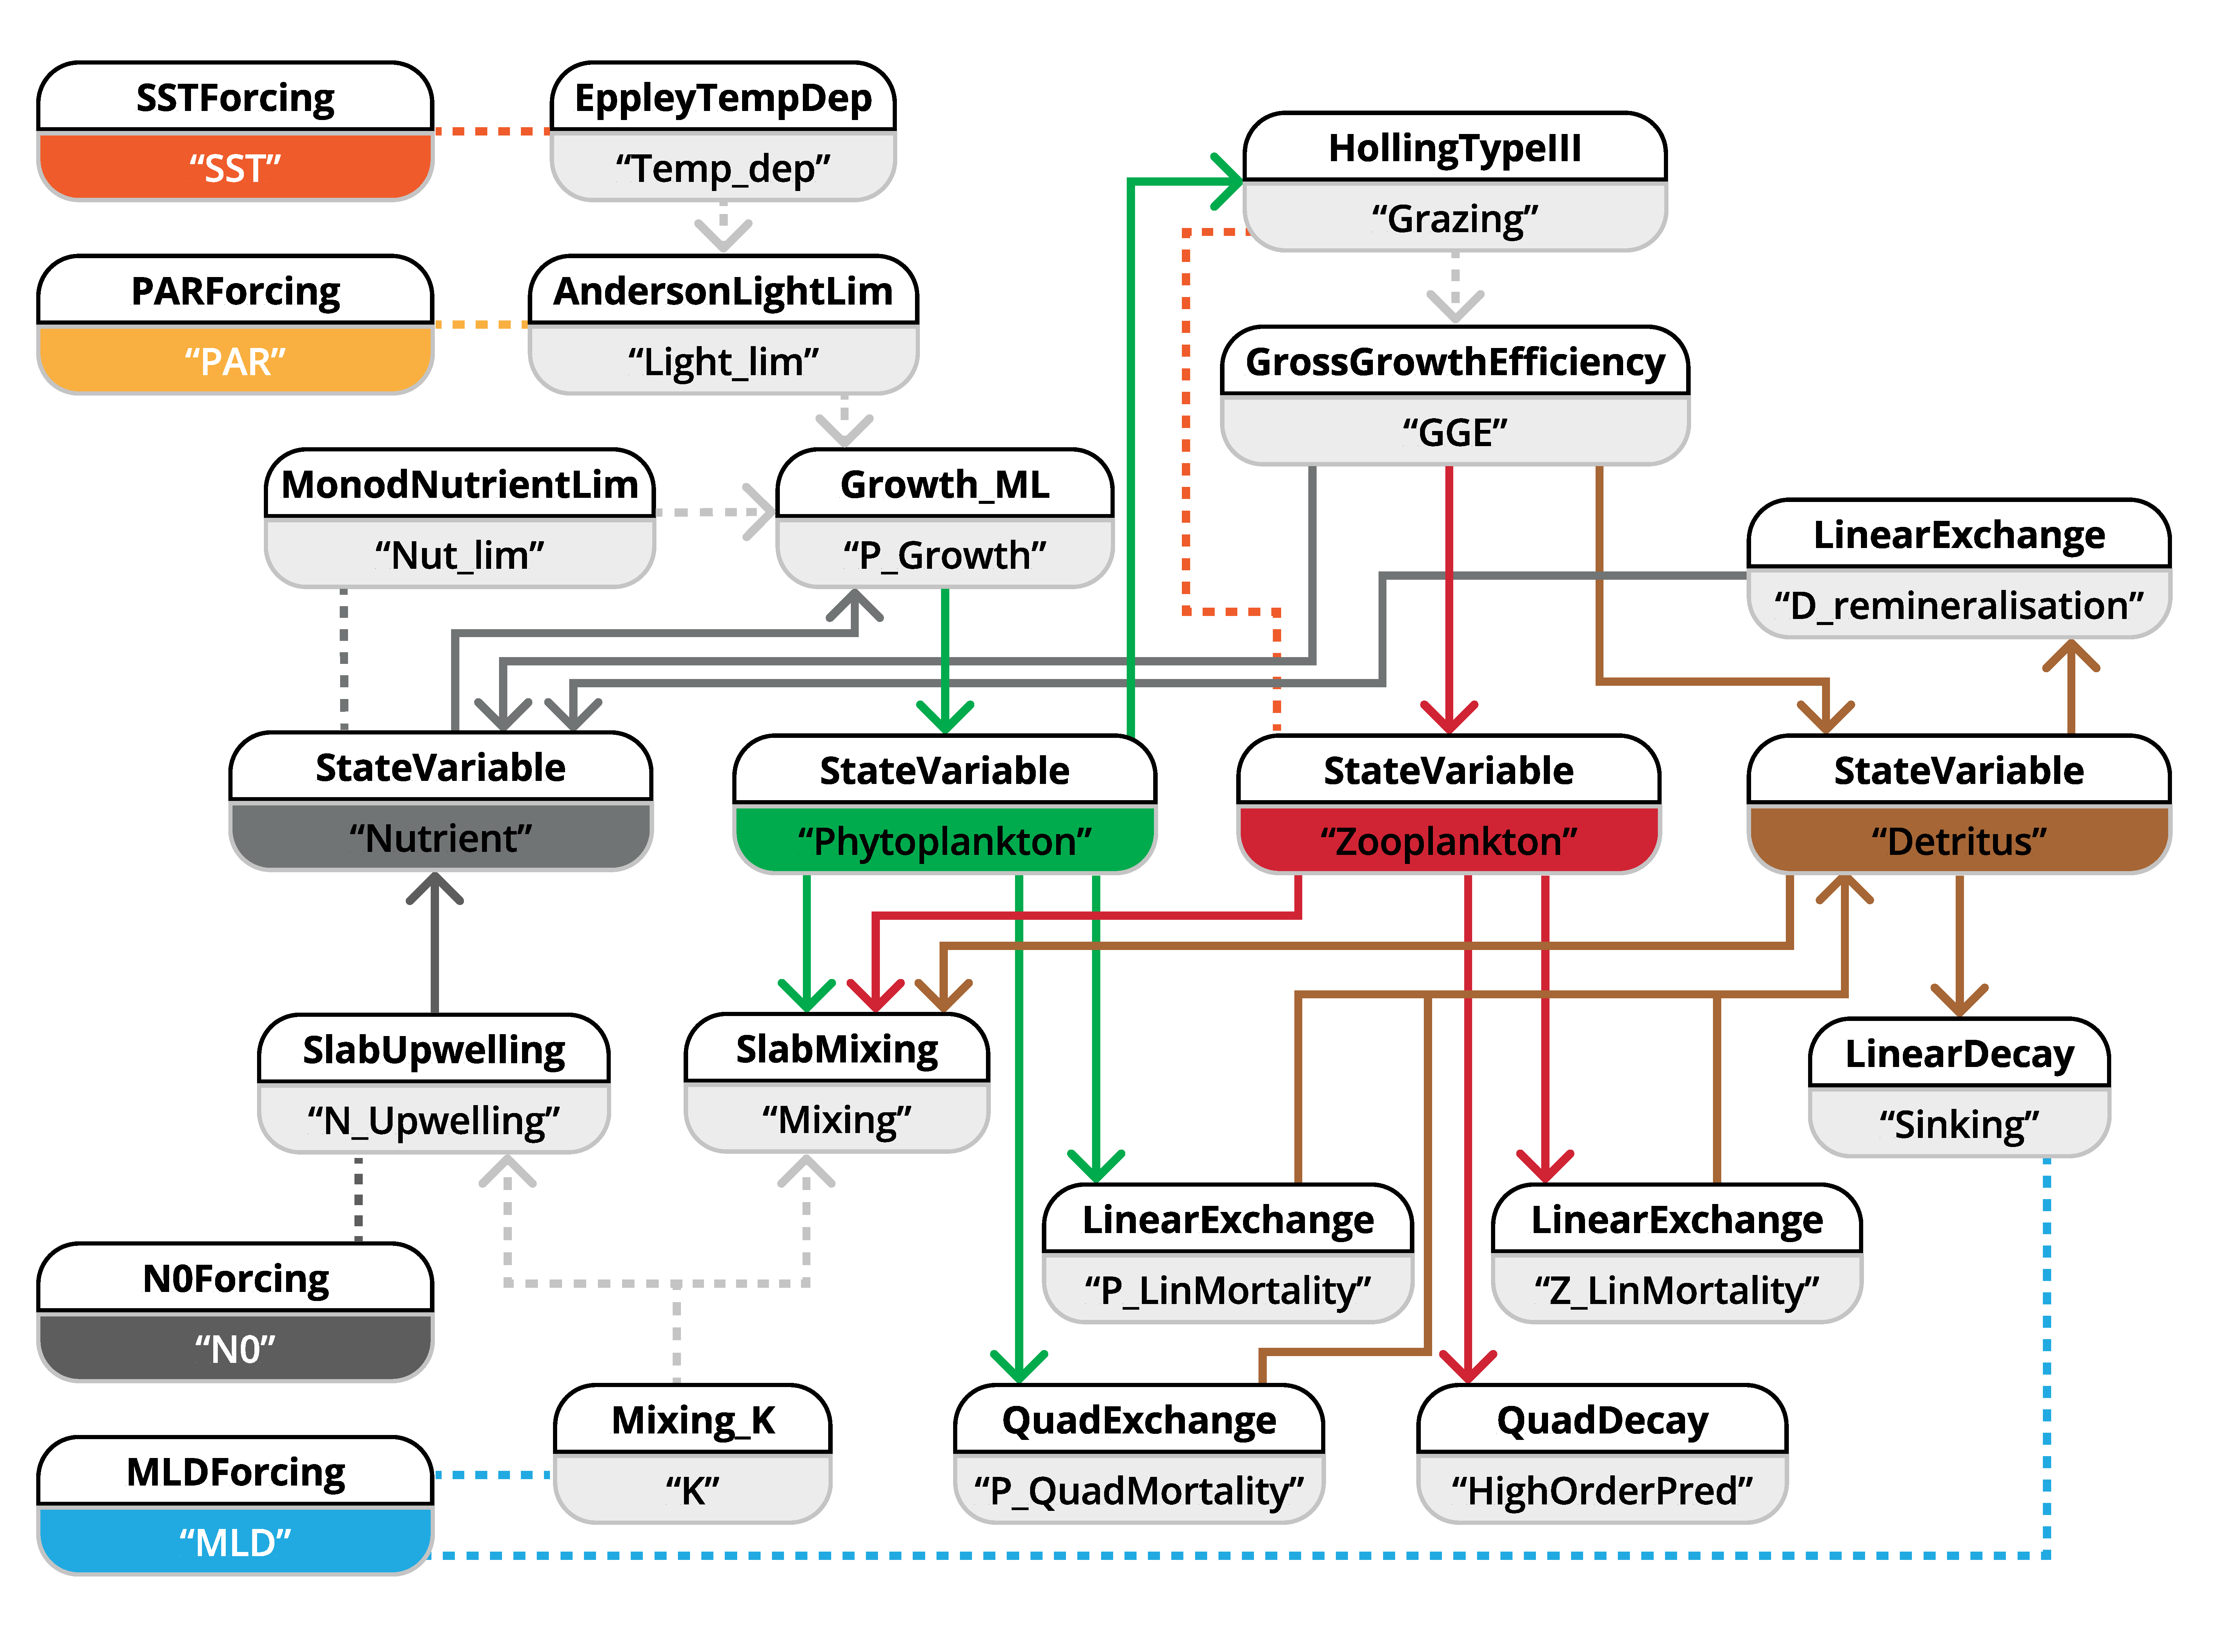
\includegraphics[width=15cm]{Figures/firstdraft_schematics/code_schematics/EMPOWER.pdf}
\caption{A schematic representation of how we implemented the NPZD slab-ocean model (application 2) in the XSO framework to include in the Phydra library. To simplify visualization, only the XSO components with their labels and links are shown. Each component contains various variables, forcings, or parameters. Solid arrows indicate the flow of fluxes between state variables. Dashed arrows indicate fluxes passed along as group variables. Dashed lines connecting processes indicate variables and forcings referenced in another component via their label.}
\label{Figure:CodeSchematics_2}
\end{figure*}

%%% TWO-COLUMN TABLE
%
%t
\begin{table*}[t]
\caption{Model parameters used in runs for use case 2 for the four stations:}
\begin{tabular}{l c c c c c r}
\tophline
Description & Parameter & BIOTRANS & India & Papa & KERFIX & Units \\
\middlehline

Max. rate of photosynthesis at 0 \unit{\degree C} & $V_P^{max}(0)$ & 2.5 & 2.5 & 1.25 & 1.25 & \unit{g C (g chl)^{-1} h^{-1}}\\
Initial slope of P-I curve & $\alpha$ & 0.15 & 0.15 & 0.075 & 0.075 & \unit{g C (g chl)^{-1} h^{-1} (W m^{-2})^{-1}}\\
Half-saturation constant for N uptake & $k_N$ & 0.85  & 0.85  & 0.85  & 0.85 & \unit{µM \ N} \\
Linear P mortality & $m_P$ & 0.015 & 0.015 & 0.015 & 0.015  & \unit{d^{−1}} \\
Quadratic P mortality & $m_{P2}$ & 0.025 & 0.025 & 0.025 & 0.025 & \unit{(µM \ N)^{-1} d^{−1}} \\
Z max. ingestion rate & $\mu_Z$ & 1.0 & 1.0 & 1.25 & 2.0 & \unit{d^{−1}} \\
Z half-saturation for intake & $k_Z$ & 0.6 & 0.6 & 0.6 & 0.6 & \unit{µM \ N} \\
Grazing preference: P & $\varphi_P$ & 0.67 & 0.67 & 0.67 & 0.67 & dimensionless\\
Grazing preference: D & $\varphi_D$ & 0.33 & 0.33 & 0.33 & 0.33 & dimensionless\\
Z absorption efficiency & $\beta_Z$ & 0.69 & 0.69 & 0.69 & 0.69 & dimensionless\\
Z net production efficiency & $k_{NZ}$ & 0.75 & 0.75 & 0.75 &  0.75 & dimensionless\\
Linear Z mortality & $m_Z$ & 0.02 & 0.0 & 0.02 & 0.02 & \unit{d^{−1}} \\
Quadratic Z mortality & $m_{Z2}$ & 0.34 & 0.34 & 0.34 & 0.34 & \unit{(µM \ N)^{-1} d^{−1}}  \\
D linear sinking rate & $v_D$ & 6.43 & 6.43 & 6.43 & 6.43 & \unit{m \ d^{−1}}\\
D remineralisation rate & $m_D$ & 0.06 & 0.06 & 0.06 & 0.06 & \unit{d^{−1}} \\
Constant mixing parameter & $\kappa$ & 0.13 & 0.13 & 0.13 & 0.13 & \unit{m \ d^{−1}}\\
Carbon-to-Chlorophyll ratio & $\theta_{chl}$ &  75 & 75 & 75 & 75 & \unit{g C \ (g Chl)^{−1}} \\

\bottomhline
\end{tabular}
\label{Table:EMPOWERparams}
\belowtable{Parameters used in the model runs for the four stations. These are optimized parameters, adapted from \citet{Anderson2015c}, that we employ to recreate their results. For consistency in this manuscript, we modified the mathematical symbols.} % Table Footnotes
\end{table*}
%

%%f
\begin{figure*}[t]
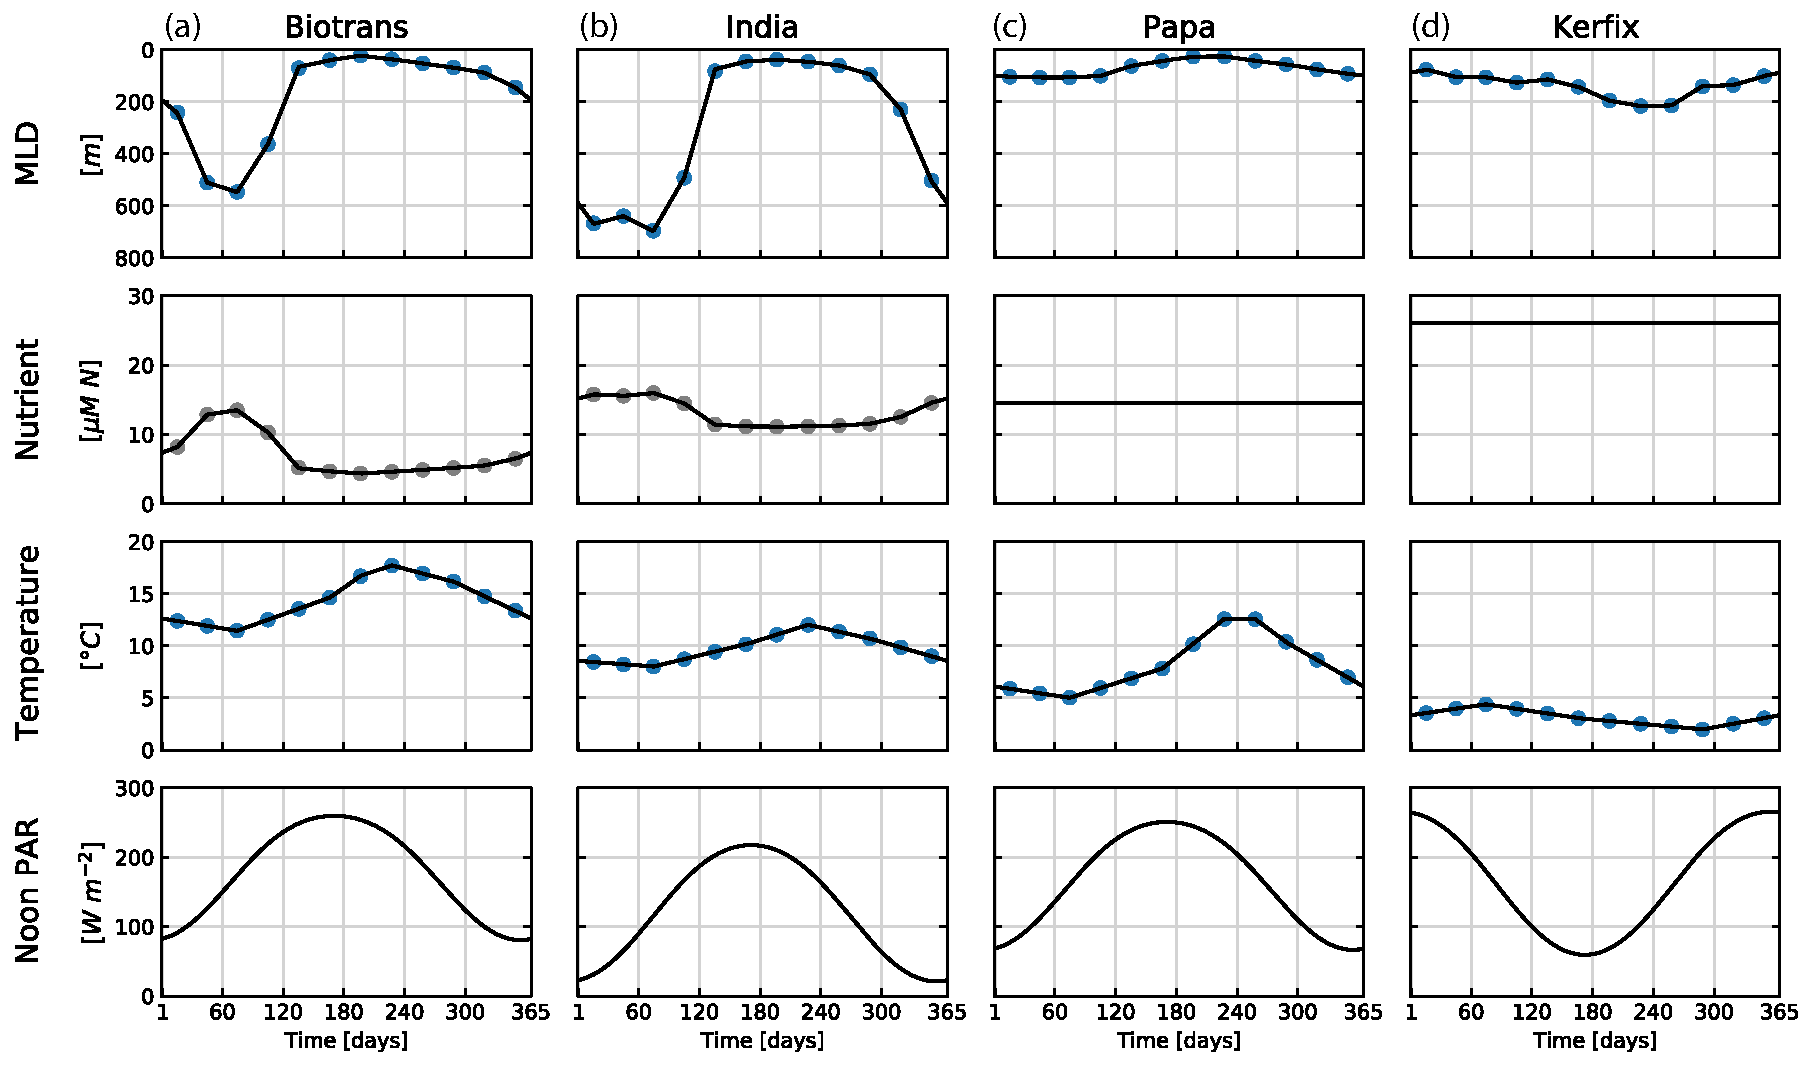
\includegraphics[width=15cm]{Figures/firstdraft_plots/02_EMPOWER_forcing.pdf}
\caption{Forcing corresponding to the four locations considered for the model application 2. Mixed Layer Depth ($H$), Nitrate below the Mixed Layer ($N_0$), irradiance at surface ($I$), and temperature averaged through the upper mixed layer ($T$). Forcing data is taken from the IFREMER MLD climatology \citep{DeBoyerMontegut2004} and WOA 2018 data \citep{Garcia2019WORLDSilicate}. The mixed layer depth (MLD) and the temperature data are extracted from up-to-date data sources corresponding to the original sources of Anderson et al. (2015). The blue dots indicate data extracted from a monthly climatology, the grey dots are calculated values from this data. Nutrient forcing is a function of depth for locations Biotrans and India and a constant value for Papa and Kerfix. Irradiance is calculated as a function of latitude.}
\label{Figure:EMPOWERforcing}
\end{figure*}

The ecological description of our model system is adapted from the EMPOWER model, however the technical implementation using the XSO framework is quite different from the procedural R script of \citet{Anderson2015c}. Instead of using hard-coded flags to choose different ecological formulations, the XSO component structure provides open modularity and interchangeability. The XSO framework defines functions irrespective of the specific time-step used for evaluation and logically separates the solving algorithm from the model formulation into the XSO backend. This allows formulating the model irrespective of the rather complex nested for-loop structure used in the original R implementation.

The amount of fluxes and interdependencies between the calculations in this application require a more elaborate component structure. As for the previous model application, we first separate the model into state variables, forcing, and fluxes.  State variables include nutrient ($N$), phytoplankton ($P$), zooplankton ($Z$), and detritus ($D$). Forcing to the model are the upper mixed layer depth ($H$), nutrient concentration below the upper mixed layer ($N_0$), temperature in the upper mixed layer ($T$), and irradiance at surface ($I$). The model defines ten unique fluxes: Phytoplankton growth, zooplankton grazing, nutrient upwelling, mixing, sinking, remineralisation, and four mortality terms.

In implementing this model within the XSO framework, we aim to find a balance between component refactoring and structural simplicity. Our goal is to allow for every ecologically relevant term to be exchangeable, whilst making full use of XSO's flexible dimensionality features. This resulted in the structure presented in figure \ref{Figure:CodeSchematics_2}.
To highlight one aspect, each factor affecting phytoplankton growth was defined by an individual component. The "group to argument" feature of the XSO framework allows for such a setup to remain highly modular, since the output of each flux with the appropriate label is utilized in the product of growth limiting terms. 
Similarly, the component calculating the mixing coefficient $K$, is computed only once and passed along to two other components, one to calculate nutrient upwelling and the other computing mixing loss fluxes of phytoplankton, zooplankton and detritus. A user could readily add more growth limiting terms via new components or exchange the component calculating $K$ without necessitating any changes to rest of the model or workflow.


Following \citet{Anderson2015c}, compare model performance in four locations representing named ocean stations: BIOTRANS, India, Papa, and KERFIX. We present the parameters in table  \ref{Table:EMPOWERparams}, which were optimized for the specific locations. Two of the stations are located in the temperate North Atlantic, BIOTRANS (47°N, 20°W) and India (60°N, 20°W), both of which exhibit a characteristic spring bloom of phytoplankton, followed by a relatively oligotrophic system over the summer. The other two stations, Papa in the North Pacific (50°N, 145°W) and KERFIX in the Southern Ocean (50°40'S, 68°25'E), represent High-Nutrient-Low-Chlorophyll (HNLC) regions with a much less pronounced seasonal cycle. The contrasting environments are apparent in the resulting model forcing data (see figure \ref{Figure:EMPOWERforcing})
In each location, the NPZD slab model is forced by four corresponding environmental factors. 
The forcing for the Mixed Layer Depth ($H$) is taken from an updated version of the IFREMER MLD climatology  \citep{DeBoyerMontegut2004} including more data and using an optimized estimation of MLD (supplied on request).
The nutrient concentration below the mixed layer ($N_0$) is calculated from a combination of the MLD climatology and depth-resolved climatology for nitrate in the World Ocean Atlas (WOA) 2018 \citep{Garcia2019WORLDSilicate}. The temperature of the mixed layer ($T$) was similarly calculated using the MLD climatology and the temperature data of WOA 2018 \citep{Locarnini2019WorldTemperature}. The monthly climatological forcing data was interpolated to be used as model forcing. For comparability, we follow \citet{Anderson2015c} in linearly interpolating the forcing.
The forcing for irradiance at surface ($I$) is calculated via a light submodel that employs trigonometric/astronomical equations to calculate light climatology for a location, given the latitude and cloud fraction as input parameters. The specific model used here and presented in \citet{Anderson2015c} was adapted from \citet{Shine1984ParametrizationAlbedo}.

To highlight another technical aspect, we used the batch dimension feature of the XSO model setup function to run the model for all four stations in parallel. This feature allows us to define a new dimension at model setup and to supply a list of values for a specific parameter. In our case, this additional dimension defines the four stations via the specific forcing and the parameters $V_P^{max}$, $\alpha$, $\mu_Z$ and $m_Z$, which are varied between locations (see table \ref{Table:EMPOWERparams}). At runtime, the model is solved for each set of parameters in the supplied lists and outputs are returned in a single Xarray dataset. The model outputs for each station can then be easily retrieved via the supplied batch dimension label (in this case \texttt{"station"}). This feature is also very useful for exploring parameter ranges, e.g. for sensitivity analysis.

We additionally show a modification of the model: \citet{Anderson2015c} included a detailed discussion of the treatment of light in a slab model. From the formulations presented in the original paper we considered two implementations. These were the simple Beer's law, which parameterizes light attenuation with a single attenuation coefficient for the whole upper mixed layer (see equation \ref{EQ:beerslaw}), and the more elaborated piecewise description, which evaluates light attenuation in three discrete depth intervals within the upper mixed layer, with specific polynomial coefficients for each interval (see equation \ref{EQ:piecewiselight}). Model results for both formulations are compared below.

\subsubsection{Results \& Discussion}
%%f
\begin{figure*}[t]
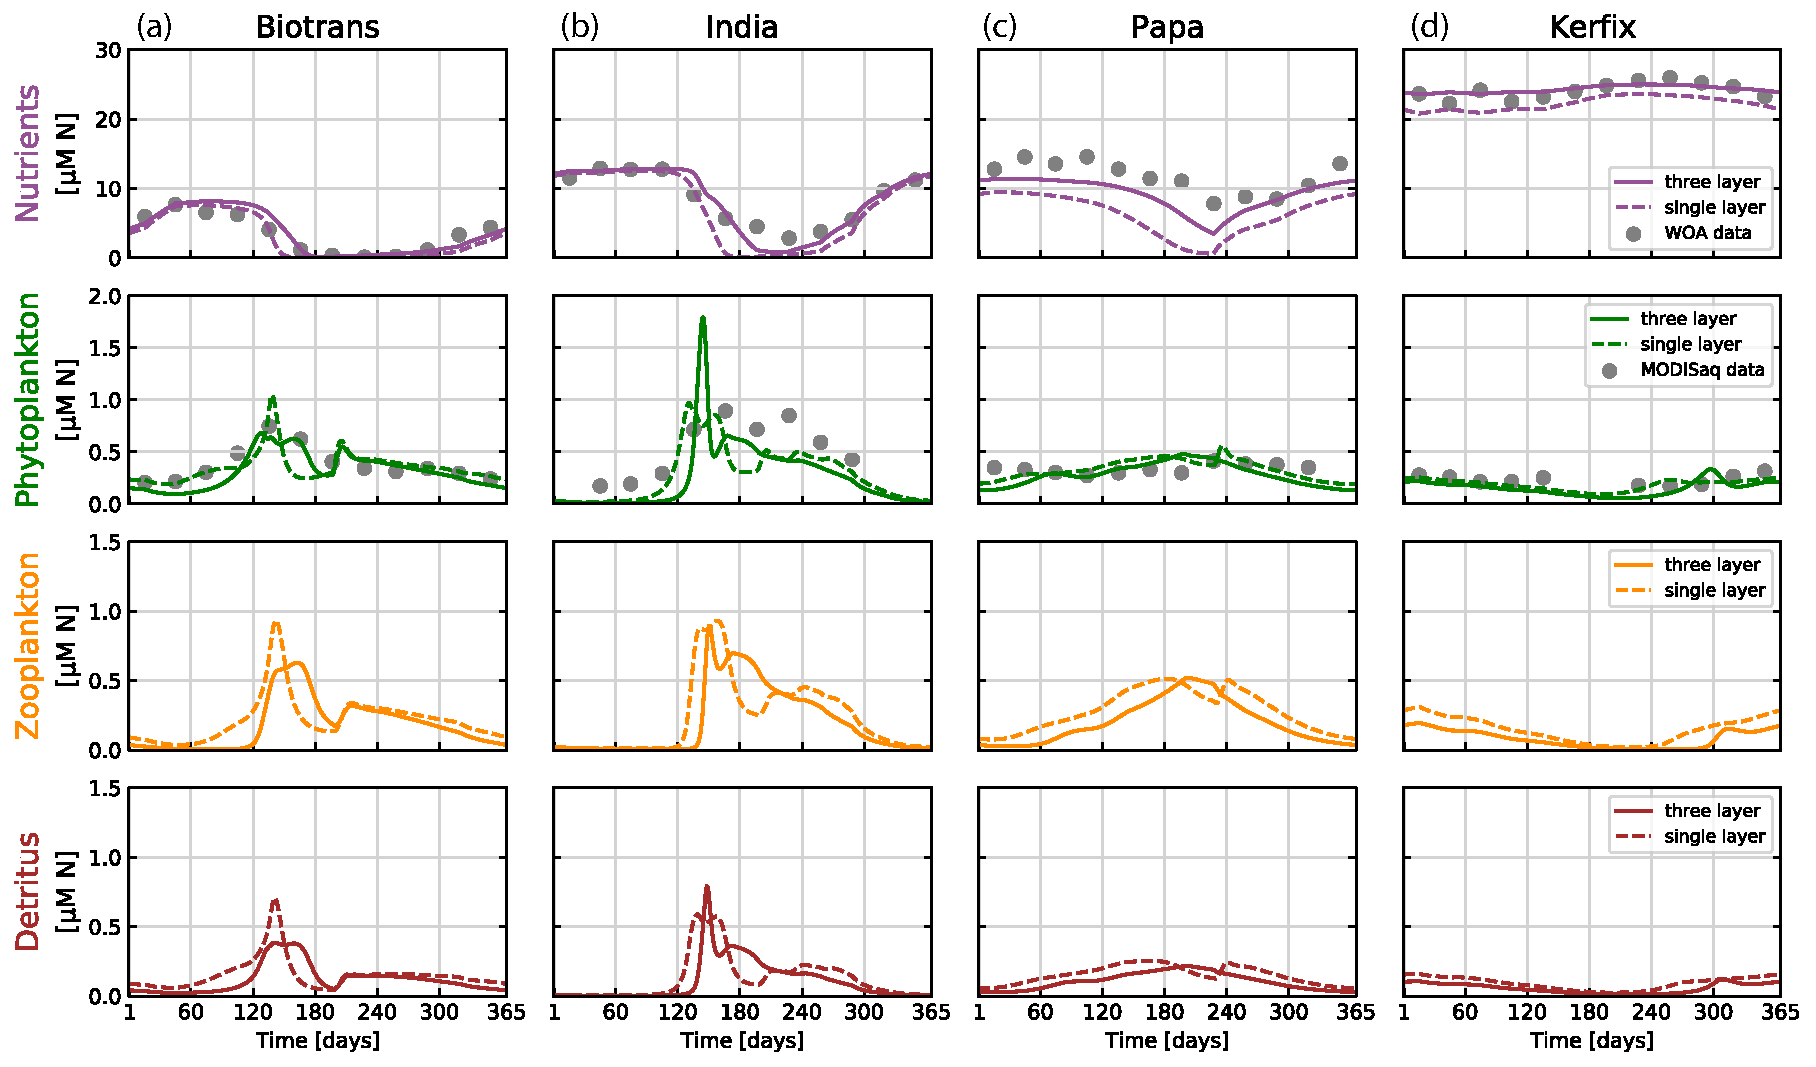
\includegraphics[width=15cm]{Figures/firstdraft_plots/02_EMPOWER_lightcomp.pdf}
\caption{Results of the NPZD model (application 2) for locations (a) BIOTRANS, (b) India, (c) Papa, and (d) KERFIX. We show here the final year of a five-year run, allowing for ample model spin-up. Model output is shown for two model variants in the light attenuation algorithm used, with everything else being kept equal (see parameters in table \ref{Table:EMPOWERparams}). The dashed line shows model output using the simple Beer's law for light attenuation (calculated over the entire mixed layer). The solid line is output from the model variant that resolves light attenuation over three discrete depth layers. The data for nitrogen in the upper mixed layer (grey dots) are extracted from WOA 2018 data, using IFREMER MLD climatology. Phytoplankton nitrogen biomass (grey dots) is calculated via $\theta_{chl}$ and Redfield ratios from MODIS Aqua chlorophyll monthly climatologies for the specific locations. Due to the locations of stations Papa, India and KERFIX, there is no satellite data coverage for some months.}
\label{Figure:ResultsEMPOWER}
\end{figure*}


Model outputs for all state variables at the four stations are shown in Figure \ref{Figure:ResultsEMPOWER}, with nutrient being compared to estimates of nitrogen concentration in the upper mixed layer, and phytoplankton concentration compared against estimates of Chlorophyll concentration from satellite data.
There is a marked seasonal cycle visible with a clear spring phytoplankton bloom for stations BIOTRANS and India, as would be expected from their location in the temperate North Atlantic. Stations Papa and KERFIX show less pronounced seasonal cycles, but still some variation, with generally higher phytoplankton and zooplankton concentrations in summer (in their respective hemisphere). Zooplankton and detritus dynamics clearly follow phytoplankton concentrations, as would be expected.

Following \citet{Anderson2015c}, the model output is compared to seasonal data for nitrate within the upper mixed layer and chlorophyll concentration at all four stations. In order to simplify the presentation, all units are given as concentration of Nitrogen \unit{µM N}. The chlorophyll concentration data was converted by a constant factor $\theta_{chl}$ (75 \unit{g C \ (g Chl)^{−1}}) and the Redfield ratio of 6.625 \unit{mol C (mol N)^{-1}} as assumed C:N of phytoplankton. We used updated versions of the original data sources to retrieve the verification data. Nitrate within the upper mixed layer is calculated from a combination of the WOA 2018 nitrate data and the IFREMER MLD Climatology used for the $N_0$ forcing. Phytoplankton concentration is compared to converted chlorophyll data from MODIS Aqua chlorophyll climatology \citep{NASAGoddardSpaceFlightCenterOceanEcologyLaboratoryOceanBiologyProcessingGroup}. We use climatology data, because we do not assume to be able to replicate particular biomass peaks of certain years with climatological forcing. The climatological data follows the general pattern shown in the chlorophyll data used as verification data in the original paper, which was taken from a specific representative year.

In general the model output agrees relatively well with our verification data, which is not surprising, since we used already optimized parameters from \citet{Anderson2015c}. 
Interestingly the change in light attenuation treatment has a pronounced effect on nutrient dynamics, as well as some effect on phytoplankton growth. The model results obtained with light attenuated according to the three-layer formulation show a better agreement with the data, particularly for station Papa. Nutrient draw-down during growth periods is consistently lower when compared to the simple Beer's law. This is caused by a greater effect of phytoplankton concentration on the resulting $k_{PAR}$ (light attenuation factor).

These results show that our framework can recreate accurately of a more complex published marine ecosystem model within a flexible and modular environment, which allows further experimentation and testing of different model structures.
Since our main aim with this model implementation was to recreate the results of \citet{Anderson2015c}, we will not go into further discussion, and gladly refer the reader to their publication for an in-depth analysis.






\subsection{Model application 3: a size-based Nutrient-Phytoplankton-Zooplankton (NPZ) model}

Our third model application is a complex size-structured plankton community model in an idealized physical setting, similar to a chemostat. The presented model is an adaptation of the ASTroCAT model, developed by Neil Banas \citep{Banas2011b}. ASTroCAT was developed as a tool to investigate the complex trophic interactions between phytoplankton and zooplankton in a systematic simplified setting, resolving a diverse plankton community via a size spectrum. Cell or organism size is used in this type of model as a "master trait", defining the parameters of specific plankton types via allometric functions, taken from literature \citep{Litchman2008}. This allows for a functional and quantifiable model to investigate mechanisms affecting and sustaining phytoplankton diversity.
Whereas Banas considered model dynamics under variable forcing or with stochastic grazing parameters, we focus here on the basic setup under constant forcing. The model, defined in the context of a chemostat, features an allometric description of multiple size-classes for phytoplankton growing on a single nutrient and zooplankton grazing on phytoplankton. While trophic interactions between size classes are highly resolved, other ecological processes are neglected (e.g. there are no detrital or regeneration pathways).  

This model lends itself well to highlight the flexibility of the XSO framework. A state variable defined within a \textit{component} can be defined with dimensions, so that it can represent an array of state variables of flexible size, as long as dimension labels match across interacting \textit{components}. The size of the state variable array depends on the number of values supplied at model setup. The built-in vectorization allows the model to compute correctly and efficiently, even with large numbers of state variables. We showcase this feature by running the model with 2 to 50 size classes and comparing bulk phytoplankton biomass between runs. The only modification necessary is varying the number of values supplied at model setup.

\subsubsection{Description}
%%f
\begin{figure}[t]
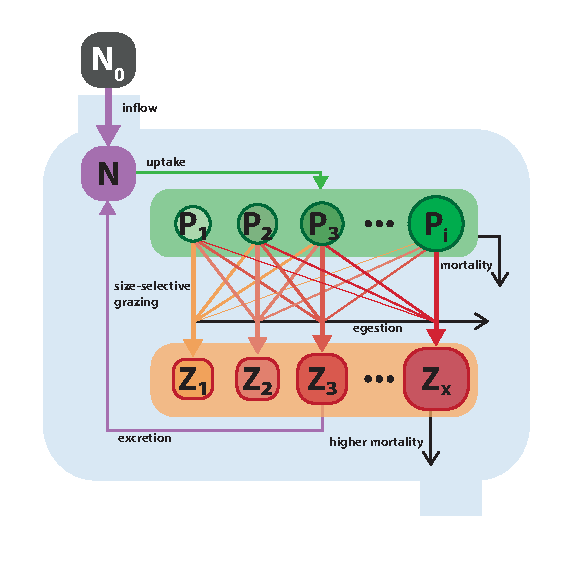
\includegraphics[width=8.3cm]{Figures/firstdraft_schematics/03_schematics_ASTroCAT.pdf}
\caption{Schematic of the size-resolved $NP_{i}Z_{j}$ trophic model. Model structure and parameterisation are adapted from \citet{Banas2011b}. 
Boxes with black and white labels represent state variables and external forcing, respectively. Arrows indicate fluxes between state variables. The blue boundary contains the ecosystem model, with state variables for a nutrient, as well as multiple size classes of phytoplankton and zooplankton. Filled arrows represent exchanges between state variables, while open arrows represent fluxes that are lost from the model system.}
\label{Figure:ModelSchematics_3}
\end{figure}

The model uses nitrogen as currency (state variables are expressed in units of \unit{µM \ N}). The physical setting is analogous to a chemostat with constant nutrient inflow counterbalanced by permanent losses. There is no constant outflow of state variables implemented, but mortality and egestion fluxes are simply lost from the system. 

The model describes a size-structured community of phytoplankton and zooplankton, whose sizes are expressed in terms of Equivalent Spherical Diameter (ESD). In line with \citet{Banas2011b}, we run our initial simulations with 40 size classes of equally log-spaced $P$ (1 to 20 \unit{\mu m}), and 40 size classes of $Z$ (2.1 to 460  \unit{\mu m}). Additionally, we perform an experiment in which the number of size classes within these ranges is varied from 2 to 50. The model can be defined with any number of size classes within meaningful boundaries of allometric relationships. Size classes are denoted by the subscript $i$ for phytoplankton and $j$ for zooplankton.

%\subsubsection{Nutrient}
Model nutrient $N$ (\unit{µM \ N}) is resupplied from an external source with concentration $N_0$ (\unit{µM \ N}) delivered at a constant rate $f$ (\unit{d^{-1}}). In addition, a fraction of grazed biomass that is not assimilated by $Z$ (units) is returned to the nutrient pool. The only loss term for $N$ is phytoplankton nutrient uptake.

\begin{equation}
    \frac{d N}{d t} = 
    f \ N_0 % Nutrient mixing
    +  (1- \epsilon - f_{eg}) \ \sum_{j} \sum_{i} G_P^{ij} % Unassimilated grazing by Z
    - \sum_{i} ( \mu_{max}^i \ \gamma_i^N \ P_i) % Phytoplankton gains
\end{equation}

%\subsubsection{Phytoplankton}
Each phytoplankton size class $P_i$ (\unit{µM \ N}) grows according to Michaelis-Menten kinetics:

\begin{equation}
    \gamma_i^N =  \frac{N}{k_N^i + N} 
\end{equation}

where $\gamma_i^N$ is the limitation on phytoplankton growth due to nutrients, $k_N^i$ (\unit{µM \ N}) is the size-dependent half saturation nutrient concentration, and $N$ is the ambient nutrient concentration.

Phytoplankton loss due to natural mortality and excretion is described with the factor $m^P$ (units) that is scaled by the maximum intrinsic growth rate $\mu_{max}^i$ (\unit{d^{-1}}), so that $m^P \mu_{max}^i$ yields the specific mortality rate for each size class.

%PHYTOPLANKTON
\begin{equation}
    \frac{d P_i}{d t} =
    \mu_{max}^i \  \gamma_i^N \   P_i  % Phytoplankton gains
    - m_P  \ \mu_{max}^i \ P_i % Linear mortality
    - \sum_{j} G_P^{ij} % Z grazing
\end{equation}


%\subsubsection{Zooplankton}
The grazing of the zooplankton size class $Z_j$ (\unit{µM \ N}) on the phytoplankton size class $P_i$ is calculated by
\begin{equation}
    G_P^{ij} = \mu_j^Z \ \frac{ \varphi_{ij} \cdot P_i }{ k_Z + \sum_{i}(\varphi_{ij} \cdot P_i) } \ Z_j
\end{equation}
where $\mu_Z^j$ (\unit{d^{-1}}) is the size-dependent maximum ingestion rate, $k_Z$ (\unit{µM \ N}) is the half-saturation level and $\varphi_{ij}$ (dimensionless) is the relative preference of $Z_j$ for $P_i$.

Prey preference is assumed to vary with phytoplankton size $size_{P}^i$ (\unit{µm}) in a log-Gaussian distribution around an optimal prey size for each grazer $size_{opt}^j$ (\unit{µm}).
\begin{equation}
    \varphi_{ij} = exp \left[ -\left( \ \frac{ log_{10}(size_P^i) - log_{10}(size_{opt}^j) }{ \Delta size_{P} } \right) \right]
\end{equation}
Where $\Delta size_{P}$ is the prey size tolerance parameter, with units of \unit{log_{10}(\mu m) ESD}, that controls the width of the Gaussian distribution.

Zooplankton growth is calculated as the product between total biomass grazed ($G_P$) and gross growth efficiency ($\epsilon$), for which values between 0.2 and 0.3 have been observed for a wide range of zooplankton \citep{Straile1997GrossGroup}. A fraction $f_{eg}$ of grazed biomass is assumed to be quickly excreted to $N$ and another fraction ($\epsilon$) that would feed into a detrital pool is permanently lost out of the system. Following \citet{Banas2011b}, the grazing fractions are split equally  so that $\epsilon = f_{eg} = 1/3$.

Zooplankton experience quadratic losses according to the parameter $m_{Z2}$. This term describes higher-order mortality and predation on zooplankton and is permanently removed from the system.

%ZOOPLANKTON
\begin{equation}
    \frac{d Z_j}{d t} =
    \epsilon \ \sum_{i} G_P^{ij} % Assimilated grazing
    - m_{Z2} \ Z_j \ \sum_{j} Z_j  % Quadratic mortality
\end{equation}


\subsubsection{Implementation}
%%f
\begin{figure*}[t]
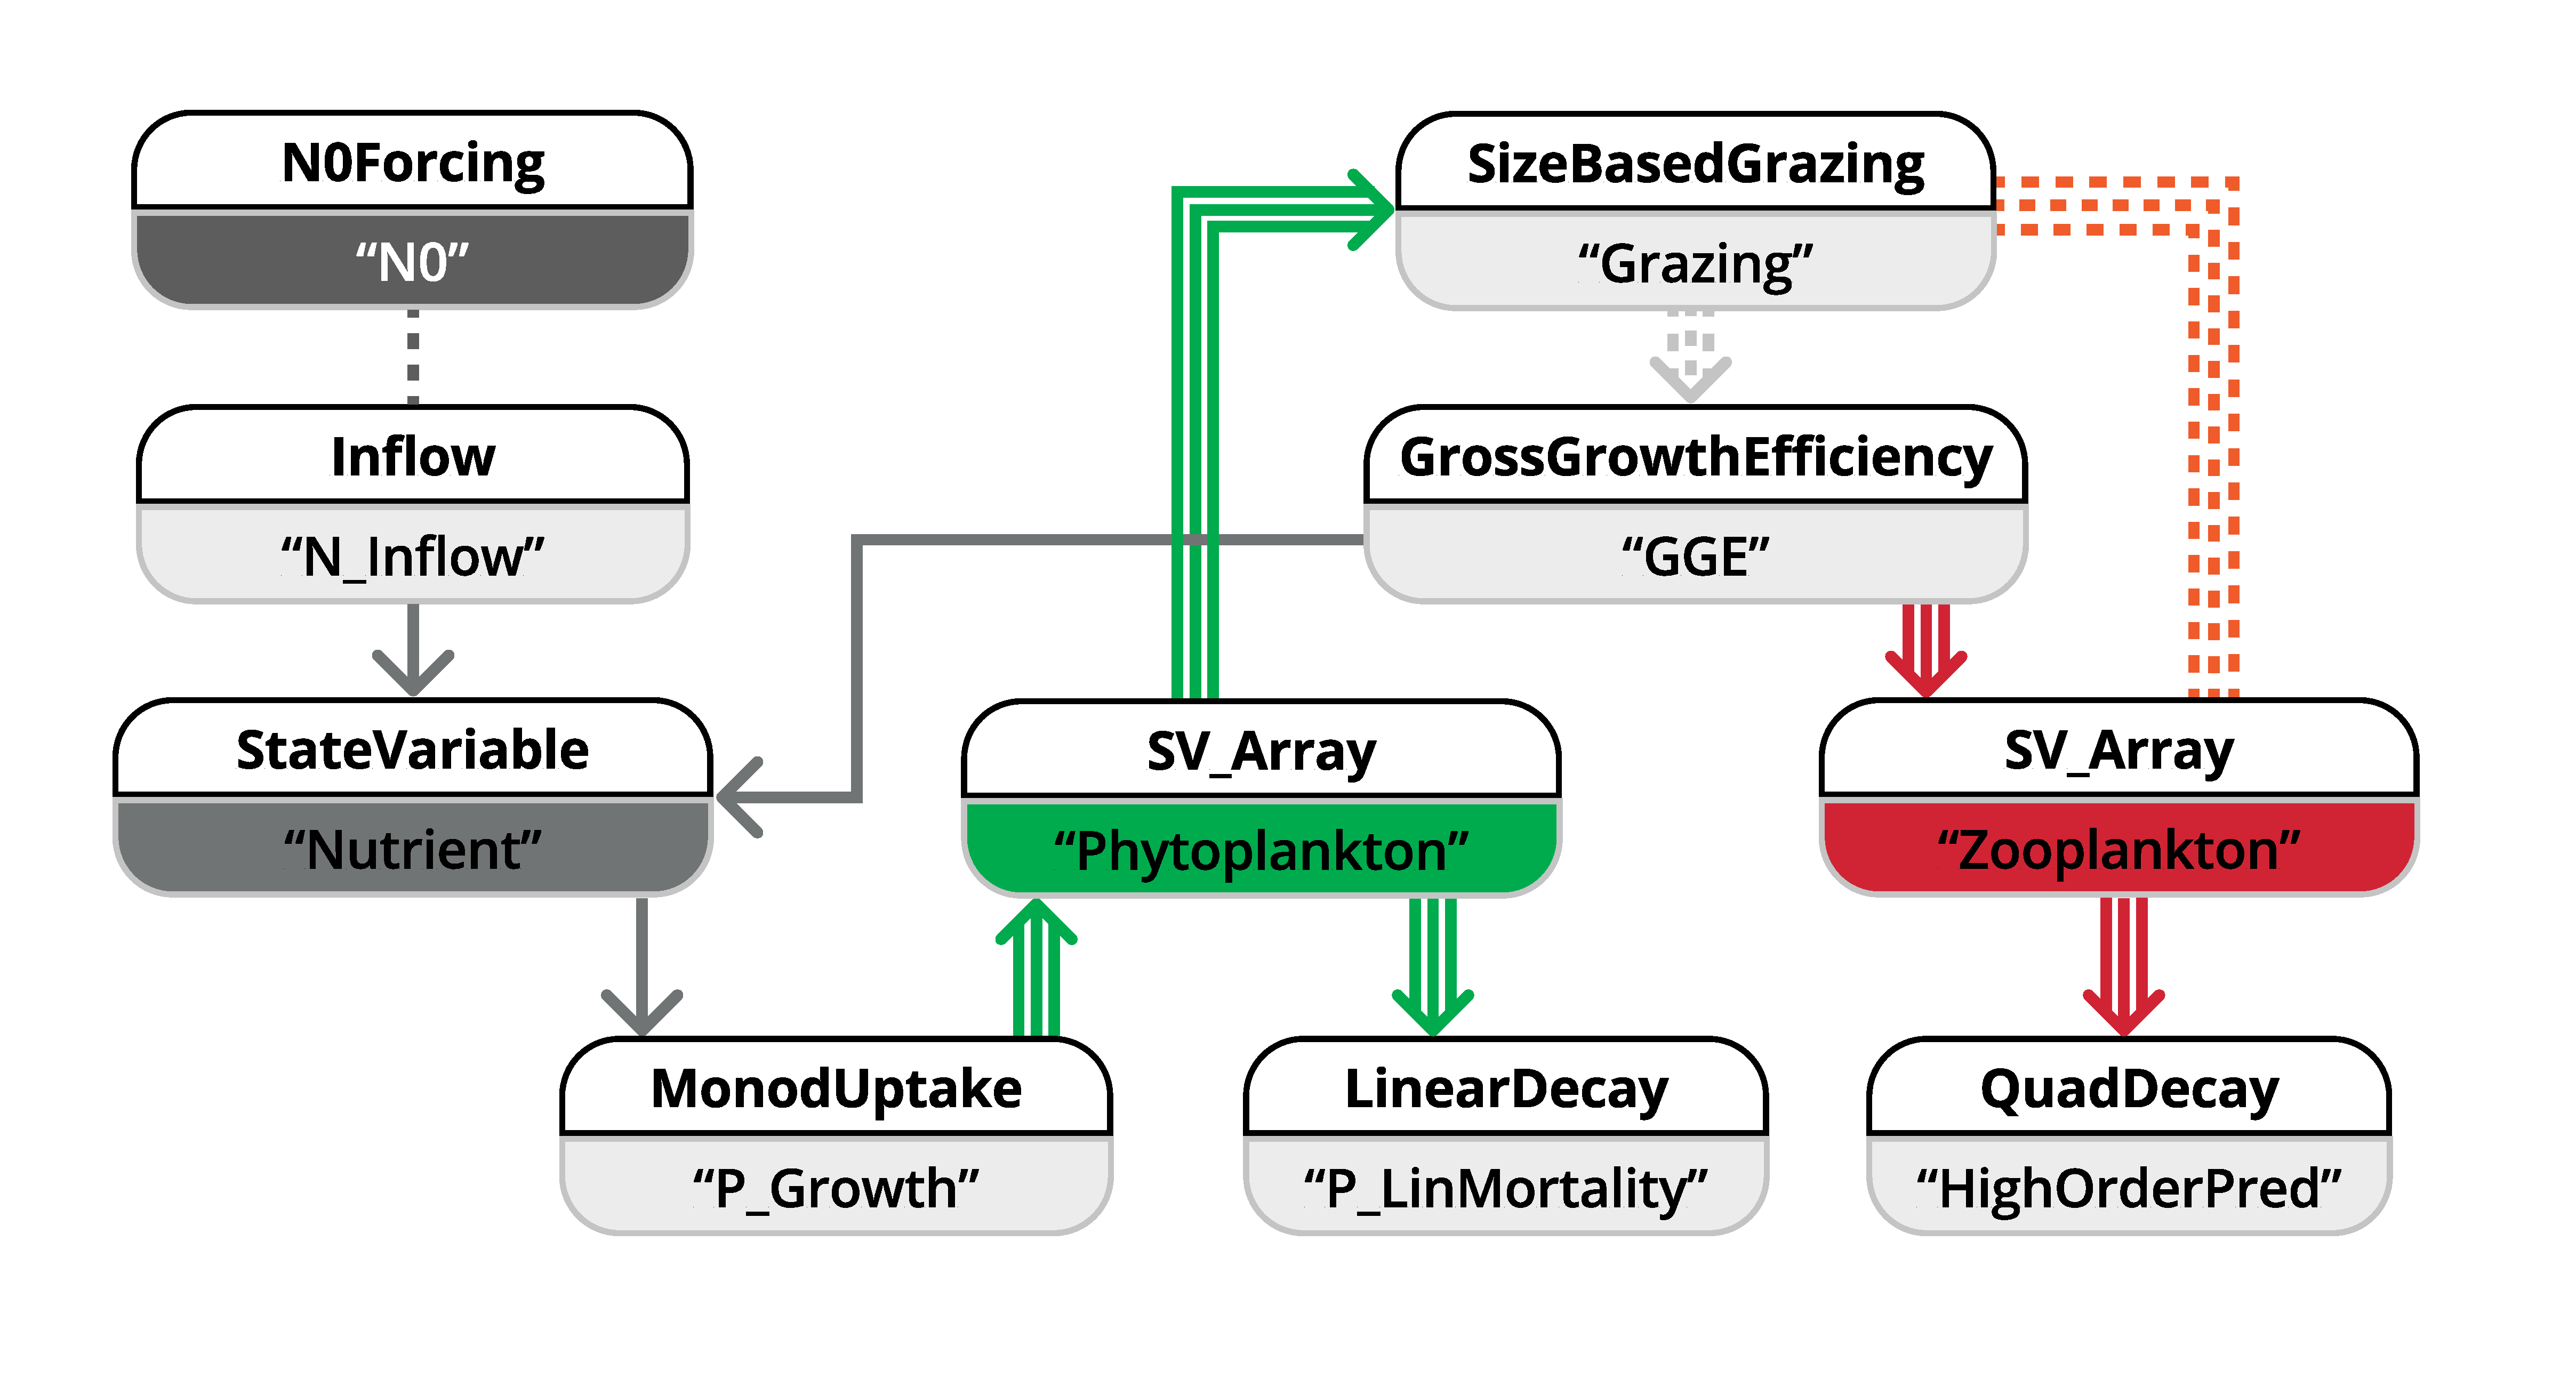
\includegraphics[width=15cm]{Figures/firstdraft_schematics/code_schematics/ASTroCAT.pdf}
\caption{A schematic representation of how model application 3 is implemented in the XSO framework and included in the Phydra library. For simplicity, only the XSO components with corresponding labels and links are shown. Each component consists of a number of variables, forcing, or parameters. Solid arrows indicate the fluxes between state variables. Dashed arrows indicate fluxes passed along as group variables. Dashed lines connecting processes indicate variables and forcing passed along via their label. Arrows with multiple lines indicate values with dimensions that are passed along.}
\label{Figure:CodeSchematics_3}
\end{figure*}


Parameters were adapted from \citet{Banas2011b}, see table \ref{Table:usecase3parameters} for all used parameter values and allometric relationships.
\begin{table*}[t]
\caption{Parameters and allometric functions used in use case 3.}
\begin{tabular}{l c c r}
Description & Parameter & Value & Units \\
\tophline
Flow rate of external nutrient & $f$ & 1 & \unit{d^{-1}} \\
External nutrient concentration & $N_0$ & 1 & \unit{µM \ N} \\
Prey half-saturation constant & $k_Z$ & 3 & \unit{µM \ N}\\
Prey size tolerance & $\Delta size_{P}$ & 0.25 & \unit{log_{10} \ \mu m}\\
Mortality fraction of $\mu_{max}^i$ for $P_i$ & $m_P$ & 0.1 & \unit{d^{-1}}\\
Zooplankton growth efficiency & $\epsilon$ & 0.33 & dimensionless\\
Fraction of grazing egested & $f_{eg}$ & 0.33 & dimensionless\\
\\

Maximum growth rate of $P_i$ &  $\mu_{max}^i$ & $ 2.6 \left( \frac{size_i^{P}}{1\mu m} \right)^{-0.45}$  & \unit{d^{-1}} \\
Nutrient half-saturation constant of $P_i$ & $k_N^i$ &  $ 0.1 \left( \frac{size_i^{P}}{1\mu m} \right)$ & \unit{µM \ N} \\

Maximum ingestion rate of $Z_j$ &  $\mu_Z^j$ & $26 \left( \frac{size^i_{P}}{1\mu m} \right)^{-0.4}$ & \unit{d^{-1}} \\

Optimum prey size of $Z_j$ & $size_{opt}^j$ &  $0.65 \left( \frac{size_{P}^i}{1\mu m} \right)^{0.56}$ & \ \unit{µm} \\

\bottomhline
\end{tabular}
\belowtable{Parameters adapted form \citet{Banas2011b}. Sources for allometric functions: \citep{Tang1995TheRespiration, Eppley1969HalfSaturationPhytoplankton, Hansen1997ZooplanktonRange, Hansen1994a}} % Table Footnotes
\label{Table:usecase3parameters}
\end{table*}
%


We separate the model into state variables, forcing, and fluxes. State variables are the nutrient ($N$), multiple size-classes of phytoplankton ($P_i$), and multiple size-classes of zooplankton ($Z_j$). The only forcing is the external nutrient input ($N_0$). At least 5 fluxes (of variable dimensionality based on the number of Zooplankton and Phytoplankton) can be defined: The inflow of the external medium, $P_i$ growing on $N$, $Z_j$ grazing on $P_i$, and mortality terms for $P_i$ and $Z_j$.
The model was implemented using 10 XSO components (Figure \ref{Figure:CodeSchematics_3}). We simplify the schematic by only showing the components with their respective labels.

The original ASTroCAT model was implemented with an interactive graphical user interface showing animations of model outputs. Our implementation in the XSO framework is technically quite similar to the original model code, with major differences being the modular component structure and the use of vectorization (instead of for-loops) to define functions computing the \textit{fluxes} acting on arrays of size-classes.

\citet{Banas2011b} presented a detailed analysis of model output for variable metrics of ecosystem complexity. We recreated a part of the analysis with a simple comparison of model dynamics for a variable number of phytoplankton and zooplankton size classes. The number of state variables can be varied at model setup by supplying a list of initial values with the desired dimensions. We ran the model for the range of 2 to 50 size classes.

\subsubsection{Results \& Discussion}
%%f
\begin{figure}[t]
\includegraphics[width=8.3cm]{Figures/firstdraft_plots/03_ASTroCAT_N50P50Z.pdf}
\caption{Nutrient concentration and plankton biomass under steady nutrient forcing obtained with model run resolving 50 phytoplankton and zooplankton size classes. Size classes are log-spaced in a range of 1 to 20 \unit{µ m} for phytoplankton and 2.16 to 420 \unit{µ m} for zooplankton. (a) Nutrient concentration over time. (b) Phytoplankton biomass by size class over 10 years of model time evolution. (c) Zooplankton biomass over the same period.}
\label{Figure:ResultsASTroCAT_1}
\end{figure}

Running the model with 40 size classes of phytoplankton and zooplankton recreates the dynamics presented by \citet{Banas2011b}. See Figure \ref{Figure:ResultsASTroCAT_1} for the time evolution of $N$, $P_i$ and $Z_j$ over a ten-year run. The size-resolved food-web shows oscillatory changes in biomass with periods from days to years, despite the much faster growth rates in the model. There appear to be tradeoffs between size classes, driven by the selective grazing interactions between zooplankton and phytoplankton. This however does not lead to chaotic behavior, but instead tends towards a stable state past 5 year of the model run. Interestingly, the general dynamics, as well as the stable state is highly clustered into some size classes. As \citet{Banas2011b} discussed, this "banding" seems to be a direct result of the prey preferences. A general conclusion one can draw, is that selective grazing interactions can be a strong factor in structuring diverse plankton communities.


%%f
\begin{figure}[t]
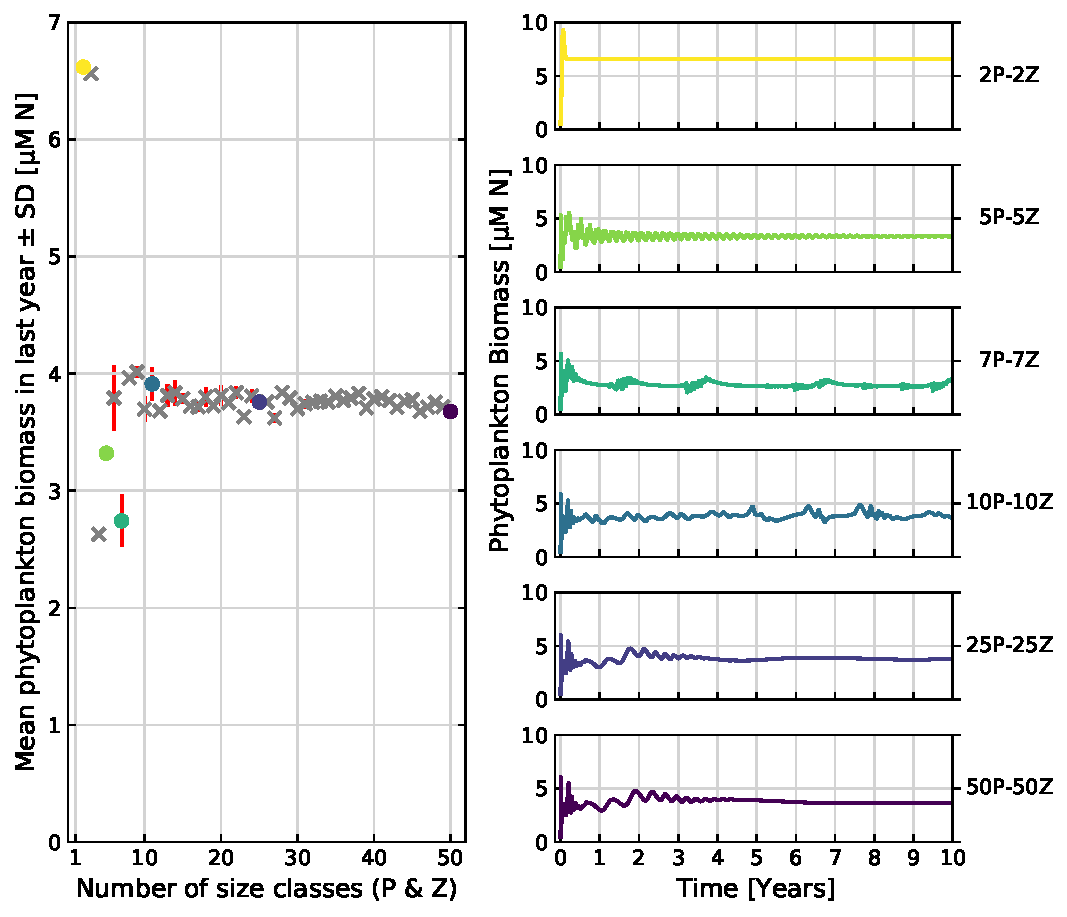
\includegraphics[width=8.3cm]{Figures/firstdraft_plots/03_ASTroCAT_sizeclassrange.pdf}
\caption{Comparative runs of our implementation of the ASTroCAT model with varying numbers of size-classes of Phytoplankton and Zooplankton. (a) Mean biomass of phytoplankton in the last year of a ten-year run for a range of 2 to 50 size classes of phytoplankton and zooplankton. Standard deviation is plotted in red. Grey crosses mark runs not otherwise shown, colored dots correspond to exemplary runs. (b) Exemplary model runs. The sum of phytoplankton biomass is shown over a ten-year run.}
\label{Figure:ResultsASTroCAT_2}
\end{figure}

To investigate the effect of the number of resolved size classes on the model output, we conducted comparative model runs varying the number of Phytoplankton and Zooplankton between 2 and 50.
Figure \ref{Figure:ResultsASTroCAT_2} shows the effect on bulk phytoplankton biomass when running the model with a variable number of size classes. A lower number of size classes (2-10) show highly variable outputs. Bulk dynamics seems to stabilize for numbers of size classes above 10. However, there are still deviations between runs in relation to the average phytoplankton biomass when more than 10 size classes are considered. The increased size resolution seems to reduce the perturbations carried on from initial model conditions, confirming the patterns observed by \citet{Baird2010IncreasingErrors}.



\section{Discussion}
% keep discussion simple! just mention a few important points!
% what is absolutely necessary?

% Andrew: Paragraph about why XSO and Phydra are needed --> overarching philosophy
We argue that plankton ecosystem model code is often built to run, but not built to be reused or understood, which is in part an issue with the programming languages and tools used to create them. This is in contrast to current tools for data analysis (e.g. in the Python and R programming language community), that are constantly developed further in a collaborative open-source effort and focus on modularity, usability, and clear documentation.
The XSO framework is an effort to provide a tool that bridges this divide, by supporting highly flexible and reproducble ODE-based modeling workflows using Python. The first release of the Phydra library contains two published plankton ecosystem models, the Empower model by \citet{Anderson2015c} and the ASTRoCAT model by \citet{Banas2011b}, that can be readily explored and modified.


\subsection{Structuring complex marine ecosystem models in a flexible framework}

% framework flexibility trade-off (design choices)
There has been an increasing move towards developing and using frameworks, that systematize or simplify at least one specific aspect of model development (e.g. FABM for model coupling, \citet{Bruggeman2014a}). However, their usage is quite scattered in the scientific community \citep{Janssen2015ExploringPerspective}. The design choices of a modeling framework have a profound effect on both the flexibility and usability, with an inherent trade-off between these two aspects. In developing the Phydra library, we went through many iterations, with the logical conclusion being the separation of the framework and library aspects.

% flexibility in model construction
Our goal in developing the framework was to allow users to build models without restricting the level of complexity, in particular in relation to the dimensionality, number of state variables and model processes. This was implemented in the framework by providing \textit{variable types}, which directly correspond to the basic mathematical components of models based on ordinary differential equations (e.g. state variables, parameters, forcing, and partial equations). Every aspect of the model needs to be defined at the level of \textit{variable types}. Model \textit{components} can be flexibly constructed from the provided set of \textit{variable types} and wrap a logical component of the model as users see fit. State variables, forcing and parameters need to be initialized in one \textit{component}, but can be referenced across the model. The system of differential equations is constructed from the \textit{fluxes} contained in the model \textit{components} via the supplied labels at model setup. These design choices make the effort required to construct models proportional to the desired model complexity, and \textit{components} can be easily modified to more complex formulations. In order to provide a template for utilizing this flexible framework, we present fully implemented models in the Phydra library. We hope that this will foster experimentation and inter-comparison of model performance at variable levels of complexity.

In addition to flexible model construction, we wanted to provide an interface for iterative modification and prototyping. An ecosystem model tracks chemical compounds as well as organisms via state variables. These state variables can define completely different components of a model, or represent a functional groups. In the third model application, we presented such a case by defining an array of variables for phytoplankton and zooplankton via size-based allometric functions. This flexible dimensionality of model components was designed with the current issues in marine ecosystem model in mind. The effects of different levels of complexity in the number and definition of phytoplankton functional types (PFT), for example, is not routinely tested in marine ecosystem models \citep{Franks2009}. Phydra provides a framework that allows for easy testing through flexible modification of such model complexity at model setup. 


% framework with Python backend and Python frontend
The choice of programming language has a great effect on the resulting framework. In contrast to available tools that allow building differential equation based models from a set of customizable building blocks through a graphical interface (e.g. Stella) or other frameworks that utilize a custom scripting language (e.g. via YAML files), the Phydra and XSO frontend and backend are fully implemented in a single programming language: Python. This might require a higher initial effort for users unfamiliar to Python, but we argue that the effort is worth the wealth of functionality provided by the Python scientific ecosystem. The XSO model development workflow is similar to writing standard Python codes, with the added benefit of a set of modular Python objects and attributes that automatically handle model inputs and outputs and that allow to computationally construct and run the model. This 

Since the XSO framework simply utilizes object-oriented Python, functional model \textit{components} have a basic syntax, but are otherwise flexible. The functions defining \textit{forcings} and \textit{fluxes} within \textit{components} in XSO are not restrictive in their Python syntax and can make use of external Python packages, as long as the value that is finally supplied at model runtime is compatible with the chosen solver backend. Since XSO itself is a wrapper of Xarray-simlab without hiding the underlying functionality, this further expands the possibilities for custom applications and further development of the framework. The flexibility of the underlying framework should not dissuade users less interested in technical customization, as the Phydra library provides fully functional pre-configured \textit{components} and \textit{model objects} that provide a solid foundation for marine ecosystem model development. 


% collaborative workflows:
The software presented here was designed to support collaborative model development. Scientists working with computational models do not always build the models themselves. Often, scientists use existing models and focus the work on parameterization and analysis of results obtained with model applications to specific locations. This type of use is specifically supported in our software because we equipped the Phydra library with pre-built \textit{model objects} and \textit{components}. A user can start working with models without detailed knowledge of the underlying framework and learn the basic workflow before progressing to building custom models using the XSO framework. Additionally, more advanced users can easily share custom \textit{components} or \textit{model objects} via the respective Python objects. This particular design makes our software suitable for teaching. 



\subsection{Current limitations of XSO and Phydra}
% XSO limitations
% XSO for ODEs only (by design)

The presented software packages are in the early stages of development, and as such have limited functionality. This first version of the XSO framework and Phydra library supports only mathematical models based on ordinary differential equations. In the first release, the framework functionality and library contents are strictly focused on zero-dimensional marine ecosystem models.
The first version of XSO implements a limited set of solver algorithms. These are a simple step-wise solver, an adaptive step-size solver optimized for solving a system of ODES (Scipy's \texttt{odeint}). The simple step-wise solver is the only backend that currently supports multi-model parallelism when executing multiple sets of parameters via the \textit{batch} dimensionality feature. None of the implemented solvers currently support single model parallelism and are thus not optimized for very large models (i.e. > 200 state variables).

The completely flexible reuse of components is currently not yet possible. We have implemented very flexible variable naming and flux routing, via string labels supplied at model setup. This is heavily reliant on the user supplying appropriate string labels, and currently there is no hard-coded linkage between components possible. However, the dimensionality of variables and fluxes has to be defined when defining the component and can not be changed after creating the model object. This is a limitation of the underlying Xarray-simlab framework, that could be improved upon in future development.

\subsection{Current usage and future developments}
% How to install and run Phydra?

Phydra and XSO are available individually via the package installer for Python (pip). Detailed instructions about installation and resolution of dependencies can be found in the online documentation. Since Python and the dependencies of Phydra are constantly developed, we provide instructions there on how to install a fully compatible virtual environment with the Conda package manager separate from a user standard Python installation. For interactive coding and prototyping of models using Phydra, we recommend using the Jupyter notebook environment that is available via Conda. For more complex and larger model runs on servers, Python scripts are preferable.

% underyling packages are constantly developed, Phydra will grow with them
The Xarray-simlab package that provides the basis for the XSO framework is a relatively young project and continuously under development, but this is a fruitful ground for developing and improving the functionalities of Phydra and XSO. As the XSO framework backend code is logically disconnected from the model definition and the solver backend is implemented in a flexible object-oriented manner.

% future feature development
The XSO framework in its current version allows building models quickly and dynamically from \textit{components} and provides a user interface to setup and run a model that is stored as a fully documented Xarray dataset. The Phydra library provides a set of \textit{components}, models, and example applications that showcase the usability of the framework and provide a common library for marine ecosystem modelling applications. Since the XSO framework is embedded in the larger Python scientific ecosystem, there are many possibilities to provide advanced functionality on top of the basic model development workflow currently supported. Amongst our foremost development goals are developing the solving backend further to support large models and possibly spatially multi-dimensional models. This would also require adding that functionality to the XSO frontend, and could include some connection to other frameworks in the backend code. Another important aspect would be simplifying the process of parameter optimization and sensitivity analysis. We are also working on methods for model introspection, such as graphically representing the model structure and exporting the system of equations. 
The Phydra library of \textit{components} and \textit{model objects} could be expanded beyond the three applications presented here and would allow easy comparability and reproducibility of specific model applications, as demonstrated here.

Phydra and XSO are open-source projects. The source code is fully accessible on GitHub and can be freely used and modified according to a BSD-3 license. Contributions via the GitHub platform are welcome and in fact greatly appreciated. Users can contribute in many ways by reporting bugs, submitting feedback, contributing to the development of the code or the documentation. More information on how interested users can contribute to the project is provided in the online documentation.


%%% added Section label for editing purposes, later simply use \conclusions
\section{Conclusions}
%\conclusions  %% \conclusions[modified heading if necessary]
% Place this project in the wider open science ecosystem, summarize and conclude

We presented two new Python packages that provide a flexible tool-set for marine ecosystem models based on differential equations. Phydra is a package that offers a library of pre-built models their individual building blocks (i.e. "components"), which can be combined or modified to create custom configurations. The XSO package, which is the technical foundation of Phydra, provides a user-friendly interface and a modular modeling framework for building and solving computational models based on differential equations. The XSO framework grants users granular control over state variables, parameters, forcing, and mathematical functions, while allowing each model component to remain interchangeable. Additionally, Phydra utilizes the Xarray dataset format for structuring model input and output, including metadata, allowing for easy storage, sharing, and analysis of data.

This project aims to unify the computational tools used by scientists for data analysis and visualisation in Python with a functional, flexible, and open-source modelling framework. The technical architecture is built on other open-source efforts (Xarray-simlab, Xarray, SciPy and NumPy to name a few) and could be further developed to provide an interface to more advanced domain-specific modelling frameworks such as Veros-BGCM or the FABM framework.

We presented three model applications of variable ecosystem complexity in zero-dimensional physical settings. These are contained in the first version of the Phydra library. A simple chemostat model of phytoplankton growing on a single nutrient showcases the workflow of implementing a model in the XSO framework in detail. The two following applications are implementations of previously published models that demonstrate the advanced functionality of the XSO framework. The second application is based on the EMPOWER model \citep{Anderson2015c}, a canonical open-ocean slab model that form the foundation of the field of marine ecosystem modelling. The third application is based on the ASTroCAT model \citep{Banas2011b}, which resolves complex trophic interactions within a size-resolved plankton model embedded in a simple physical flow-through setting. These three applications are contained in the Phydra library via their respective model \textit{components} and as fully assembled \textit{model objects}. Additionally, all scripts used to create the presented results are available in fully documented Jupyter notebooks in the model examples folder of the Phydra package. This should provide a foundation for users to start experimenting with the modelling framework. 

The Phydra library can be a reference and learning resource for scientists interested in marine ecosystem modelling, a starting point for scientific exploration, and a valuable tool for teaching. The model development effort is proportional to the desired complexity of the model application, so users can quickly implement simple models.

Creating such a fully integrated modeling environment for marine ecosystem models will require a diverse community of users and developers. We believe the programming language Python provides strong enough functionalities and a wide enough user base, and tried to approach the issue of granular model construction as one of earlier steps towards a wider ecosystem for integrated marine ecosystem modeling.

We hope Phydra and XSO contribute to the ongoing efforts in the community of developing more robust, transparent, and reproducible models, moving away from monolithic and inflexible codes to a model development process that is inherently collaborative. Both packages are open source and available under a BSD-3 license on GitHub.

%% END OF SECTION CONCLUSIONS







\begin{comment}


SAVED TEXT SNIPPETS::


Open source development efforts in the marine modeling community are working to improve on these issues, and have lead to great advancements by providing tools for validation 
\citep[e.g. BGCval,][]{DeMora2018BGC-val:Models} or the flexible coupling of physical and ecological models \citep[e.g. FABM,][]{Bruggeman2014a}.

In related domains, there have been efforts to create platforms, conducive to scientific collaboration utilizing Jupyter notebooks \citep[e.g.][]{Hut2022TheCollaboration}.

The open-source ERSEM marine ecosystem model provides some flexibility to modify and experiment with model structures via markup language files or Python interfaces, but the general formulations are hard-coded in Fortran scripts \citep{Butenschon2016}. 

There is the option to rewrite Fortran model code into a more modular structure, as was done in an update to the FABM-PCLake aquatic ecosystem model \citep[][]{Schnedler-Meyer2022WaterModel}. Another option is to utilize a separate modeling language, that provides some interface to a GUI or Python code \citep{Norling2021RapidV1.0}. 

Modern, interpreted programming languages commonly used for data analysis applications (e.g. Python) have evolved the capabilities to efficiently support advanced numerical computations \citep{Lin2012}. This is showcased by Veros, a global circulation model (GCM) written in Python \citep{Hafner2018VerosPython}.

\end{comment}



%% The following commands are for the statements about the availability of data sets and/or software code corresponding to the manuscript.
%% It is strongly recommended to make use of these sections in case data sets and/or software code have been part of your research the article is based on.

\codeavailability{TEXT} %% use this section when having only software code available


\dataavailability{TEXT} %% use this section when having only data sets available


\codedataavailability{TEXT} %% use this section when having data sets and software code available


\sampleavailability{TEXT} %% use this section when having geoscientific samples available


\videosupplement{TEXT} %% use this section when having video supplements available


\appendix



\noappendix       %% use this to mark the end of the appendix section. Otherwise the figures might be numbered incorrectly (e.g. 10 instead of 1).

%% Regarding figures and tables in appendices, the following two options are possible depending on your general handling of figures and tables in the manuscript environment:

%% Option 1: If you sorted all figures and tables into the sections of the text, please also sort the appendix figures and appendix tables into the respective appendix sections.
%% They will be correctly named automatically.

%% Option 2: If you put all figures after the reference list, please insert appendix tables and figures after the normal tables and figures.
%% To rename them correctly to A1, A2, etc., please add the following commands in front of them:

\appendixfigures  %% needs to be added in front of appendix figures

\appendixtables   %% needs to be added in front of appendix tables

%% Please add \clearpage between each table and/or figure. Further guidelines on figures and tables can be found below.



\authorcontribution{TEXT} %% this section is mandatory

\competinginterests{TEXT} %% this section is mandatory even if you declare that no competing interests are present

\disclaimer{TEXT} %% optional section

\begin{acknowledgements}
TEXT
\end{acknowledgements}




%% REFERENCES

%% The reference list is compiled as follows:

%\begin{thebibliography}{}

%\bibitem[AUTHOR(YEAR)]{LABEL1}
%REFERENCE 1

%\bibitem[AUTHOR(YEAR)]{LABEL2}
%REFERENCE 2

%\end{thebibliography}

%% Since the Copernicus LaTeX package includes the BibTeX style file copernicus.bst,
%% authors experienced with BibTeX only have to include the following two lines:
%%
\bibliographystyle{copernicus}
\bibliography{references.bib}
%%
%% URLs and DOIs can be entered in your BibTeX file as:
%%
%% URL = {http://www.xyz.org/~jones/idx_g.htm}
%% DOI = {10.5194/xyz}


%% LITERATURE CITATIONS
%%
%% command                        & example result
%% \citet{jones90}|               & Jones et al. (1990)
%% \citep{jones90}|               & (Jones et al., 1990)
%% \citep{jones90,jones93}|       & (Jones et al., 1990, 1993)
%% \citep[p.~32]{jones90}|        & (Jones et al., 1990, p.~32)
%% \citep[e.g.,][]{jones90}|      & (e.g., Jones et al., 1990)
%% \citep[e.g.,][p.~32]{jones90}| & (e.g., Jones et al., 1990, p.~32)
%% \citeauthor{jones90}|          & Jones et al.
%% \citeyear{jones90}|            & 1990



%% FIGURES

%% When figures and tables are placed at the end of the MS (article in one-column style), please add \clearpage
%% between bibliography and first table and/or figure as well as between each table and/or figure.

% The figure files should be labelled correctly with Arabic numerals (e.g. fig01.jpg, fig02.png).


%% ONE-COLUMN FIGURES

%%f
%\begin{figure}[t]
%\includegraphics[width=8.3cm]{FILE NAME}
%\caption{TEXT}
%\end{figure}
%
%%% TWO-COLUMN FIGURES
%
%%f
%\begin{figure*}[t]
%\includegraphics[width=12cm]{FILE NAME}
%\caption{TEXT}
%\end{figure*}
%
%
%%% TABLES
%%%
%%% The different columns must be seperated with a & command and should
%%% end with \\ to identify the column brake.
%
%%% ONE-COLUMN TABLE
%
%%t
%\begin{table}[t]
%\caption{TEXT}
%\begin{tabular}{column = lcr}
%\tophline
%
%\middlehline
%
%\bottomhline
%\end{tabular}
%\belowtable{} % Table Footnotes
%\end{table}
%
%%% TWO-COLUMN TABLE
%
%%t
%\begin{table*}[t]
%\caption{TEXT}
%\begin{tabular}{column = lcr}
%\tophline
%
%\middlehline
%
%\bottomhline
%\end{tabular}
%\belowtable{} % Table Footnotes
%\end{table*}
%
%%% LANDSCAPE TABLE
%
%%t
%\begin{sidewaystable*}[t]
%\caption{TEXT}
%\begin{tabular}{column = lcr}
%\tophline
%
%\middlehline
%
%\bottomhline
%\end{tabular}
%\belowtable{} % Table Footnotes
%\end{sidewaystable*}
%
%
%%% MATHEMATICAL EXPRESSIONS
%
%%% All papers typeset by Copernicus Publications follow the math typesetting regulations
%%% given by the IUPAC Green Book (IUPAC: Quantities, Units and Symbols in Physical Chemistry,
%%% 2nd Edn., Blackwell Science, available at: http://old.iupac.org/publications/books/gbook/green_book_2ed.pdf, 1993).
%%%
%%% Physical quantities/variables are typeset in italic font (t for time, T for Temperature)
%%% Indices which are not defined are typeset in italic font (x, y, z, a, b, c)
%%% Items/objects which are defined are typeset in roman font (Car A, Car B)
%%% Descriptions/specifications which are defined by itself are typeset in roman font (abs, rel, ref, tot, net, ice)
%%% Abbreviations from 2 letters are typeset in roman font (RH, LAI)
%%% Vectors are identified in bold italic font using \vec{x}
%%% Matrices are identified in bold roman font
%%% Multiplication signs are typeset using the LaTeX commands \times (for vector products, grids, and exponential notations) or \cdot
%%% The character * should not be applied as mutliplication sign
%
%
%%% EQUATIONS
%
%%% Single-row equation
%
%\begin{equation}
%
%\end{equation}
%
%%% Multiline equation
%
%\begin{align}
%& 3 + 5 = 8\\
%& 3 + 5 = 8\\
%& 3 + 5 = 8
%\end{align}
%
%
%%% MATRICES
%
%\begin{matrix}
%x & y & z\\
%x & y & z\\
%x & y & z\\
%\end{matrix}
%
%
%%% ALGORITHM
%
%\begin{algorithm}
%\caption{...}
%\label{a1}
%\begin{algorithmic}
%...
%\end{algorithmic}
%\end{algorithm}
%
%
%%% CHEMICAL FORMULAS AND REACTIONS
%
%%% For formulas embedded in the text, please use \chem{}
%
%%% The reaction environment creates labels including the letter R, i.e. (R1), (R2), etc.
%
%\begin{reaction}
%%% \rightarrow should be used for normal (one-way) chemical reactions
%%% \rightleftharpoons should be used for equilibria
%%% \leftrightarrow should be used for resonance structures
%\end{reaction}
%
%
%%% PHYSICAL UNITS
%%%
%%% Please use \unit{} and apply the exponential notation


\end{document}
